%%%%%%%%%%%%%%%%%%%%%%%%%%%%%
%ES100 Latex Template
%Sam Meijer '19
%Hopefully this template will serve you well.
%It is built off many other packages and templates, but I have added my own style here and there, as you should too!
%I will endeavour to explain some of the intricacies of LaTex as well as how to lay out an overall project.
%Hopefully no knowledge of LaTex is required to understand this document.
%I would highly recommend https://www.overleaf.com/learn/latex/Main_Page for further information.
%For errata, please contact smeijer11@gmail.com.
%%%%%%%%%%%%%%%%%%%%%%%%%%%%%

%Packages are included below, these are akin to libraries in other programming languages. As far as I can tell, there is no reason to reduce the number of packages included in a document. It might compile faster, but overleaf compiles fast so this should not be an issue.
\documentclass[12pt,twoside]{report} %tells the compiler that this is a 'report' style document, and the main font size.
\usepackage{setspace} %allows the use of '\doublespace' to set line spacing
\usepackage[utf8]{inputenc} %inclusion of this is optional, overleaf includes it in its compiler so it is not necessary, it may be necessary for other compilers.
\usepackage[english]{babel} %this does a few things eg allowing dates to be made by the compiler. probably best not to get rid of it
\usepackage{wrapfig} %if it is desirable to wrap text (see https://www.overleaf.com/learn/latex/Wrapping_text_around_figures).
\usepackage{graphicx} %this allows graphics to be put in easily
\usepackage{float}%this allows you to put them in good places
\usepackage[version=4]{mhchem} %this is good for chemical reactions
\usepackage{amsmath} %maths package
\usepackage{amssymb} %symbol package
\usepackage{textcomp,gensymb} %more symbols (eg \degree)
\usepackage{appendix} %self explanatory
\usepackage{colortbl} %good for colouring in cells on a table
\usepackage{rotating} %allows you to rotate graphics
\usepackage{bm} %helps bold things
\usepackage{multirow} %for tables
\usepackage{longtable} %for long tables
\usepackage{booktabs} %more tables
\usepackage{pdfpages} %allows PDFs to be included in document (good if you want to include a pdf in an appendix eg)
\usepackage{caption} %allows captions for graphics
\usepackage[nottoc]{tocbibind} %adds the bibliography to the table of contents
\usepackage{subcaption} %allows subcaption for multiple images in one graphic

\PassOptionsToPackage{hyphens}{url}\usepackage{hyperref}
\usepackage{hyperref} %this is great for putting hyperreferences in the document.
\usepackage[table]{xcolor} %more colouring of tables
\definecolor{Gray}{gray}{0.9} %this defines a colour to be used and gives it a name. This is a colour called 'Gray' it is 'gray' with transparency 0.9
 %%%%%%%%%%%%%%%%%%%%%%%%%%%%%%%%%%%%%%%%%%%%%%%%%%%%%%%%%%%%%%%%%%%%%%%%%%%%%%%% 
%%% ~ Arduino Language - Arduino IDE Colors ~                                  %%%
%%%                                                                            %%%
%%% Kyle Rocha-Brownell | 10/2/2017 | No Licence                               %%%
%%% -------------------------------------------------------------------------- %%%
%%%                                                                            %%%
%%% Place this file in your working directory (next to the latex file you're   %%%
%%% working on).  To add it to your project, place:                            %%%
%%%     %%%%%%%%%%%%%%%%%%%%%%%%%%%%%%%%%%%%%%%%%%%%%%%%%%%%%%%%%%%%%%%%%%%%%%%%%%%%%%%% 
%%% ~ Arduino Language - Arduino IDE Colors ~                                  %%%
%%%                                                                            %%%
%%% Kyle Rocha-Brownell | 10/2/2017 | No Licence                               %%%
%%% -------------------------------------------------------------------------- %%%
%%%                                                                            %%%
%%% Place this file in your working directory (next to the latex file you're   %%%
%%% working on).  To add it to your project, place:                            %%%
%%%     %%%%%%%%%%%%%%%%%%%%%%%%%%%%%%%%%%%%%%%%%%%%%%%%%%%%%%%%%%%%%%%%%%%%%%%%%%%%%%%% 
%%% ~ Arduino Language - Arduino IDE Colors ~                                  %%%
%%%                                                                            %%%
%%% Kyle Rocha-Brownell | 10/2/2017 | No Licence                               %%%
%%% -------------------------------------------------------------------------- %%%
%%%                                                                            %%%
%%% Place this file in your working directory (next to the latex file you're   %%%
%%% working on).  To add it to your project, place:                            %%%
%%%    \input{arduinoLanguage.tex}                                             %%%
%%% somewhere before \begin{document} in your latex file.                      %%%
%%%                                                                            %%%
%%% In your document, place your arduino code between:                         %%%
%%%   \begin{lstlisting}[language=Arduino]                                     %%%
%%% and:                                                                       %%%
%%%   \end{lstlisting}                                                         %%%
%%%                                                                            %%%
%%% Or create your own style to add non-built-in functions and variables.      %%%
%%%                                                                            %%%
 %%%%%%%%%%%%%%%%%%%%%%%%%%%%%%%%%%%%%%%%%%%%%%%%%%%%%%%%%%%%%%%%%%%%%%%%%%%%%%%% 


\usepackage{listings}    
\usepackage{courier}

%%% Define Custom IDE Colors %%%
\definecolor{arduinoGreen}    {rgb} {0.17, 0.43, 0.01}
\definecolor{arduinoGrey}     {rgb} {0.47, 0.47, 0.33}
\definecolor{arduinoOrange}   {rgb} {0.8 , 0.4 , 0   }
\definecolor{arduinoBlue}     {rgb} {0.01, 0.61, 0.98}
\definecolor{arduinoDarkBlue} {rgb} {0.0 , 0.2 , 0.5 }

%%% Define Arduino Language %%%
\lstdefinelanguage{Arduino}{
  language=C++, % begin with default C++ settings 
%
%
  %%% Keyword Color Group 1 %%%  (called KEYWORD3 by arduino)
  keywordstyle=\color{arduinoGreen},   
  deletekeywords={  % remove all arduino keywords that might be in c++
                break, case, override, final, continue, default, do, else, for, 
                if, return, goto, switch, throw, try, while, setup, loop, export, 
                not, or, and, xor, include, define, elif, else, error, if, ifdef, 
                ifndef, pragma, warning,
                HIGH, LOW, INPUT, INPUT_PULLUP, OUTPUT, DEC, BIN, HEX, OCT, PI, 
                HALF_PI, TWO_PI, LSBFIRST, MSBFIRST, CHANGE, FALLING, RISING, 
                DEFAULT, EXTERNAL, INTERNAL, INTERNAL1V1, INTERNAL2V56, LED_BUILTIN, 
                LED_BUILTIN_RX, LED_BUILTIN_TX, DIGITAL_MESSAGE, FIRMATA_STRING, 
                ANALOG_MESSAGE, REPORT_DIGITAL, REPORT_ANALOG, SET_PIN_MODE, 
                SYSTEM_RESET, SYSEX_START, auto, int8_t, int16_t, int32_t, int64_t, 
                uint8_t, uint16_t, uint32_t, uint64_t, char16_t, char32_t, operator, 
                enum, delete, bool, boolean, byte, char, const, false, float, double, 
                null, NULL, int, long, new, private, protected, public, short, 
                signed, static, volatile, String, void, true, unsigned, word, array, 
                sizeof, dynamic_cast, typedef, const_cast, struct, static_cast, union, 
                friend, extern, class, reinterpret_cast, register, explicit, inline, 
                _Bool, complex, _Complex, _Imaginary, atomic_bool, atomic_char, 
                atomic_schar, atomic_uchar, atomic_short, atomic_ushort, atomic_int, 
                atomic_uint, atomic_long, atomic_ulong, atomic_llong, atomic_ullong, 
                virtual, PROGMEM,
                Serial, Serial1, Serial2, Serial3, SerialUSB, Keyboard, Mouse,
                abs, acos, asin, atan, atan2, ceil, constrain, cos, degrees, exp, 
                floor, log, map, max, min, radians, random, randomSeed, round, sin, 
                sq, sqrt, tan, pow, bitRead, bitWrite, bitSet, bitClear, bit, 
                highByte, lowByte, analogReference, analogRead, 
                analogReadResolution, analogWrite, analogWriteResolution, 
                attachInterrupt, detachInterrupt, digitalPinToInterrupt, delay, 
                delayMicroseconds, digitalWrite, digitalRead, interrupts, millis, 
                micros, noInterrupts, noTone, pinMode, pulseIn, pulseInLong, shiftIn, 
                shiftOut, tone, yield, Stream, begin, end, peek, read, print, 
                println, available, availableForWrite, flush, setTimeout, find, 
                findUntil, parseInt, parseFloat, readBytes, readBytesUntil, readString, 
                readStringUntil, trim, toUpperCase, toLowerCase, charAt, compareTo, 
                concat, endsWith, startsWith, equals, equalsIgnoreCase, getBytes, 
                indexOf, lastIndexOf, length, replace, setCharAt, substring, 
                toCharArray, toInt, press, release, releaseAll, accept, click, move, 
                isPressed, isAlphaNumeric, isAlpha, isAscii, isWhitespace, isControl, 
                isDigit, isGraph, isLowerCase, isPrintable, isPunct, isSpace, 
                isUpperCase, isHexadecimalDigit, 
                }, 
  morekeywords={   % add arduino structures to group 1
                break, case, override, final, continue, default, do, else, for, 
                if, return, goto, switch, throw, try, while, setup, loop, export, 
                not, or, and, xor, include, define, elif, else, error, if, ifdef, 
                ifndef, pragma, warning,
                }, 
% 
%
  %%% Keyword Color Group 2 %%%  (called LITERAL1 by arduino)
  keywordstyle=[2]\color{arduinoBlue},   
  keywords=[2]{   % add variables and dataTypes as 2nd group  
                HIGH, LOW, INPUT, INPUT_PULLUP, OUTPUT, DEC, BIN, HEX, OCT, PI, 
                HALF_PI, TWO_PI, LSBFIRST, MSBFIRST, CHANGE, FALLING, RISING, 
                DEFAULT, EXTERNAL, INTERNAL, INTERNAL1V1, INTERNAL2V56, LED_BUILTIN, 
                LED_BUILTIN_RX, LED_BUILTIN_TX, DIGITAL_MESSAGE, FIRMATA_STRING, 
                ANALOG_MESSAGE, REPORT_DIGITAL, REPORT_ANALOG, SET_PIN_MODE, 
                SYSTEM_RESET, SYSEX_START, auto, int8_t, int16_t, int32_t, int64_t, 
                uint8_t, uint16_t, uint32_t, uint64_t, char16_t, char32_t, operator, 
                enum, delete, bool, boolean, byte, char, const, false, float, double, 
                null, NULL, int, long, new, private, protected, public, short, 
                signed, static, volatile, String, void, true, unsigned, word, array, 
                sizeof, dynamic_cast, typedef, const_cast, struct, static_cast, union, 
                friend, extern, class, reinterpret_cast, register, explicit, inline, 
                _Bool, complex, _Complex, _Imaginary, atomic_bool, atomic_char, 
                atomic_schar, atomic_uchar, atomic_short, atomic_ushort, atomic_int, 
                atomic_uint, atomic_long, atomic_ulong, atomic_llong, atomic_ullong, 
                virtual, PROGMEM,
                },  
% 
%
  %%% Keyword Color Group 3 %%%  (called KEYWORD1 by arduino)
  keywordstyle=[3]\bfseries\color{arduinoOrange},
  keywords=[3]{  % add built-in functions as a 3rd group
                Serial, Serial1, Serial2, Serial3, SerialUSB, Keyboard, Mouse,
                },      
%
%
  %%% Keyword Color Group 4 %%%  (called KEYWORD2 by arduino)
  keywordstyle=[4]\color{arduinoOrange},
  keywords=[4]{  % add more built-in functions as a 4th group
                abs, acos, asin, atan, atan2, ceil, constrain, cos, degrees, exp, 
                floor, log, map, max, min, radians, random, randomSeed, round, sin, 
                sq, sqrt, tan, pow, bitRead, bitWrite, bitSet, bitClear, bit, 
                highByte, lowByte, analogReference, analogRead, 
                analogReadResolution, analogWrite, analogWriteResolution, 
                attachInterrupt, detachInterrupt, digitalPinToInterrupt, delay, 
                delayMicroseconds, digitalWrite, digitalRead, interrupts, millis, 
                micros, noInterrupts, noTone, pinMode, pulseIn, pulseInLong, shiftIn, 
                shiftOut, tone, yield, Stream, begin, end, peek, read, print, 
                println, available, availableForWrite, flush, setTimeout, find, 
                findUntil, parseInt, parseFloat, readBytes, readBytesUntil, readString, 
                readStringUntil, trim, toUpperCase, toLowerCase, charAt, compareTo, 
                concat, endsWith, startsWith, equals, equalsIgnoreCase, getBytes, 
                indexOf, lastIndexOf, length, replace, setCharAt, substring, 
                toCharArray, toInt, press, release, releaseAll, accept, click, move, 
                isPressed, isAlphaNumeric, isAlpha, isAscii, isWhitespace, isControl, 
                isDigit, isGraph, isLowerCase, isPrintable, isPunct, isSpace, 
                isUpperCase, isHexadecimalDigit, 
                },      
%
%
  %%% Set Other Colors %%%
  stringstyle=\color{arduinoDarkBlue},    
  commentstyle=\color{arduinoGrey},    
%          
%   
  %%%% Line Numbering %%%%
   numbers=left,                    
  numbersep=5pt,                   
  numberstyle=\color{arduinoGrey},    
  %stepnumber=2,                      % show every 2 line numbers
%
%
  %%%% Code Box Style %%%%
  breaklines=true,                    % wordwrapping
  tabsize=2,         
  basicstyle=\ttfamily  
}                                             %%%
%%% somewhere before \begin{document} in your latex file.                      %%%
%%%                                                                            %%%
%%% In your document, place your arduino code between:                         %%%
%%%   \begin{lstlisting}[language=Arduino]                                     %%%
%%% and:                                                                       %%%
%%%   \end{lstlisting}                                                         %%%
%%%                                                                            %%%
%%% Or create your own style to add non-built-in functions and variables.      %%%
%%%                                                                            %%%
 %%%%%%%%%%%%%%%%%%%%%%%%%%%%%%%%%%%%%%%%%%%%%%%%%%%%%%%%%%%%%%%%%%%%%%%%%%%%%%%% 


\usepackage{listings}    
\usepackage{courier}

%%% Define Custom IDE Colors %%%
\definecolor{arduinoGreen}    {rgb} {0.17, 0.43, 0.01}
\definecolor{arduinoGrey}     {rgb} {0.47, 0.47, 0.33}
\definecolor{arduinoOrange}   {rgb} {0.8 , 0.4 , 0   }
\definecolor{arduinoBlue}     {rgb} {0.01, 0.61, 0.98}
\definecolor{arduinoDarkBlue} {rgb} {0.0 , 0.2 , 0.5 }

%%% Define Arduino Language %%%
\lstdefinelanguage{Arduino}{
  language=C++, % begin with default C++ settings 
%
%
  %%% Keyword Color Group 1 %%%  (called KEYWORD3 by arduino)
  keywordstyle=\color{arduinoGreen},   
  deletekeywords={  % remove all arduino keywords that might be in c++
                break, case, override, final, continue, default, do, else, for, 
                if, return, goto, switch, throw, try, while, setup, loop, export, 
                not, or, and, xor, include, define, elif, else, error, if, ifdef, 
                ifndef, pragma, warning,
                HIGH, LOW, INPUT, INPUT_PULLUP, OUTPUT, DEC, BIN, HEX, OCT, PI, 
                HALF_PI, TWO_PI, LSBFIRST, MSBFIRST, CHANGE, FALLING, RISING, 
                DEFAULT, EXTERNAL, INTERNAL, INTERNAL1V1, INTERNAL2V56, LED_BUILTIN, 
                LED_BUILTIN_RX, LED_BUILTIN_TX, DIGITAL_MESSAGE, FIRMATA_STRING, 
                ANALOG_MESSAGE, REPORT_DIGITAL, REPORT_ANALOG, SET_PIN_MODE, 
                SYSTEM_RESET, SYSEX_START, auto, int8_t, int16_t, int32_t, int64_t, 
                uint8_t, uint16_t, uint32_t, uint64_t, char16_t, char32_t, operator, 
                enum, delete, bool, boolean, byte, char, const, false, float, double, 
                null, NULL, int, long, new, private, protected, public, short, 
                signed, static, volatile, String, void, true, unsigned, word, array, 
                sizeof, dynamic_cast, typedef, const_cast, struct, static_cast, union, 
                friend, extern, class, reinterpret_cast, register, explicit, inline, 
                _Bool, complex, _Complex, _Imaginary, atomic_bool, atomic_char, 
                atomic_schar, atomic_uchar, atomic_short, atomic_ushort, atomic_int, 
                atomic_uint, atomic_long, atomic_ulong, atomic_llong, atomic_ullong, 
                virtual, PROGMEM,
                Serial, Serial1, Serial2, Serial3, SerialUSB, Keyboard, Mouse,
                abs, acos, asin, atan, atan2, ceil, constrain, cos, degrees, exp, 
                floor, log, map, max, min, radians, random, randomSeed, round, sin, 
                sq, sqrt, tan, pow, bitRead, bitWrite, bitSet, bitClear, bit, 
                highByte, lowByte, analogReference, analogRead, 
                analogReadResolution, analogWrite, analogWriteResolution, 
                attachInterrupt, detachInterrupt, digitalPinToInterrupt, delay, 
                delayMicroseconds, digitalWrite, digitalRead, interrupts, millis, 
                micros, noInterrupts, noTone, pinMode, pulseIn, pulseInLong, shiftIn, 
                shiftOut, tone, yield, Stream, begin, end, peek, read, print, 
                println, available, availableForWrite, flush, setTimeout, find, 
                findUntil, parseInt, parseFloat, readBytes, readBytesUntil, readString, 
                readStringUntil, trim, toUpperCase, toLowerCase, charAt, compareTo, 
                concat, endsWith, startsWith, equals, equalsIgnoreCase, getBytes, 
                indexOf, lastIndexOf, length, replace, setCharAt, substring, 
                toCharArray, toInt, press, release, releaseAll, accept, click, move, 
                isPressed, isAlphaNumeric, isAlpha, isAscii, isWhitespace, isControl, 
                isDigit, isGraph, isLowerCase, isPrintable, isPunct, isSpace, 
                isUpperCase, isHexadecimalDigit, 
                }, 
  morekeywords={   % add arduino structures to group 1
                break, case, override, final, continue, default, do, else, for, 
                if, return, goto, switch, throw, try, while, setup, loop, export, 
                not, or, and, xor, include, define, elif, else, error, if, ifdef, 
                ifndef, pragma, warning,
                }, 
% 
%
  %%% Keyword Color Group 2 %%%  (called LITERAL1 by arduino)
  keywordstyle=[2]\color{arduinoBlue},   
  keywords=[2]{   % add variables and dataTypes as 2nd group  
                HIGH, LOW, INPUT, INPUT_PULLUP, OUTPUT, DEC, BIN, HEX, OCT, PI, 
                HALF_PI, TWO_PI, LSBFIRST, MSBFIRST, CHANGE, FALLING, RISING, 
                DEFAULT, EXTERNAL, INTERNAL, INTERNAL1V1, INTERNAL2V56, LED_BUILTIN, 
                LED_BUILTIN_RX, LED_BUILTIN_TX, DIGITAL_MESSAGE, FIRMATA_STRING, 
                ANALOG_MESSAGE, REPORT_DIGITAL, REPORT_ANALOG, SET_PIN_MODE, 
                SYSTEM_RESET, SYSEX_START, auto, int8_t, int16_t, int32_t, int64_t, 
                uint8_t, uint16_t, uint32_t, uint64_t, char16_t, char32_t, operator, 
                enum, delete, bool, boolean, byte, char, const, false, float, double, 
                null, NULL, int, long, new, private, protected, public, short, 
                signed, static, volatile, String, void, true, unsigned, word, array, 
                sizeof, dynamic_cast, typedef, const_cast, struct, static_cast, union, 
                friend, extern, class, reinterpret_cast, register, explicit, inline, 
                _Bool, complex, _Complex, _Imaginary, atomic_bool, atomic_char, 
                atomic_schar, atomic_uchar, atomic_short, atomic_ushort, atomic_int, 
                atomic_uint, atomic_long, atomic_ulong, atomic_llong, atomic_ullong, 
                virtual, PROGMEM,
                },  
% 
%
  %%% Keyword Color Group 3 %%%  (called KEYWORD1 by arduino)
  keywordstyle=[3]\bfseries\color{arduinoOrange},
  keywords=[3]{  % add built-in functions as a 3rd group
                Serial, Serial1, Serial2, Serial3, SerialUSB, Keyboard, Mouse,
                },      
%
%
  %%% Keyword Color Group 4 %%%  (called KEYWORD2 by arduino)
  keywordstyle=[4]\color{arduinoOrange},
  keywords=[4]{  % add more built-in functions as a 4th group
                abs, acos, asin, atan, atan2, ceil, constrain, cos, degrees, exp, 
                floor, log, map, max, min, radians, random, randomSeed, round, sin, 
                sq, sqrt, tan, pow, bitRead, bitWrite, bitSet, bitClear, bit, 
                highByte, lowByte, analogReference, analogRead, 
                analogReadResolution, analogWrite, analogWriteResolution, 
                attachInterrupt, detachInterrupt, digitalPinToInterrupt, delay, 
                delayMicroseconds, digitalWrite, digitalRead, interrupts, millis, 
                micros, noInterrupts, noTone, pinMode, pulseIn, pulseInLong, shiftIn, 
                shiftOut, tone, yield, Stream, begin, end, peek, read, print, 
                println, available, availableForWrite, flush, setTimeout, find, 
                findUntil, parseInt, parseFloat, readBytes, readBytesUntil, readString, 
                readStringUntil, trim, toUpperCase, toLowerCase, charAt, compareTo, 
                concat, endsWith, startsWith, equals, equalsIgnoreCase, getBytes, 
                indexOf, lastIndexOf, length, replace, setCharAt, substring, 
                toCharArray, toInt, press, release, releaseAll, accept, click, move, 
                isPressed, isAlphaNumeric, isAlpha, isAscii, isWhitespace, isControl, 
                isDigit, isGraph, isLowerCase, isPrintable, isPunct, isSpace, 
                isUpperCase, isHexadecimalDigit, 
                },      
%
%
  %%% Set Other Colors %%%
  stringstyle=\color{arduinoDarkBlue},    
  commentstyle=\color{arduinoGrey},    
%          
%   
  %%%% Line Numbering %%%%
   numbers=left,                    
  numbersep=5pt,                   
  numberstyle=\color{arduinoGrey},    
  %stepnumber=2,                      % show every 2 line numbers
%
%
  %%%% Code Box Style %%%%
  breaklines=true,                    % wordwrapping
  tabsize=2,         
  basicstyle=\ttfamily  
}                                             %%%
%%% somewhere before \begin{document} in your latex file.                      %%%
%%%                                                                            %%%
%%% In your document, place your arduino code between:                         %%%
%%%   \begin{lstlisting}[language=Arduino]                                     %%%
%%% and:                                                                       %%%
%%%   \end{lstlisting}                                                         %%%
%%%                                                                            %%%
%%% Or create your own style to add non-built-in functions and variables.      %%%
%%%                                                                            %%%
 %%%%%%%%%%%%%%%%%%%%%%%%%%%%%%%%%%%%%%%%%%%%%%%%%%%%%%%%%%%%%%%%%%%%%%%%%%%%%%%% 


\usepackage{listings}    
\usepackage{courier}

%%% Define Custom IDE Colors %%%
\definecolor{arduinoGreen}    {rgb} {0.17, 0.43, 0.01}
\definecolor{arduinoGrey}     {rgb} {0.47, 0.47, 0.33}
\definecolor{arduinoOrange}   {rgb} {0.8 , 0.4 , 0   }
\definecolor{arduinoBlue}     {rgb} {0.01, 0.61, 0.98}
\definecolor{arduinoDarkBlue} {rgb} {0.0 , 0.2 , 0.5 }

%%% Define Arduino Language %%%
\lstdefinelanguage{Arduino}{
  language=C++, % begin with default C++ settings 
%
%
  %%% Keyword Color Group 1 %%%  (called KEYWORD3 by arduino)
  keywordstyle=\color{arduinoGreen},   
  deletekeywords={  % remove all arduino keywords that might be in c++
                break, case, override, final, continue, default, do, else, for, 
                if, return, goto, switch, throw, try, while, setup, loop, export, 
                not, or, and, xor, include, define, elif, else, error, if, ifdef, 
                ifndef, pragma, warning,
                HIGH, LOW, INPUT, INPUT_PULLUP, OUTPUT, DEC, BIN, HEX, OCT, PI, 
                HALF_PI, TWO_PI, LSBFIRST, MSBFIRST, CHANGE, FALLING, RISING, 
                DEFAULT, EXTERNAL, INTERNAL, INTERNAL1V1, INTERNAL2V56, LED_BUILTIN, 
                LED_BUILTIN_RX, LED_BUILTIN_TX, DIGITAL_MESSAGE, FIRMATA_STRING, 
                ANALOG_MESSAGE, REPORT_DIGITAL, REPORT_ANALOG, SET_PIN_MODE, 
                SYSTEM_RESET, SYSEX_START, auto, int8_t, int16_t, int32_t, int64_t, 
                uint8_t, uint16_t, uint32_t, uint64_t, char16_t, char32_t, operator, 
                enum, delete, bool, boolean, byte, char, const, false, float, double, 
                null, NULL, int, long, new, private, protected, public, short, 
                signed, static, volatile, String, void, true, unsigned, word, array, 
                sizeof, dynamic_cast, typedef, const_cast, struct, static_cast, union, 
                friend, extern, class, reinterpret_cast, register, explicit, inline, 
                _Bool, complex, _Complex, _Imaginary, atomic_bool, atomic_char, 
                atomic_schar, atomic_uchar, atomic_short, atomic_ushort, atomic_int, 
                atomic_uint, atomic_long, atomic_ulong, atomic_llong, atomic_ullong, 
                virtual, PROGMEM,
                Serial, Serial1, Serial2, Serial3, SerialUSB, Keyboard, Mouse,
                abs, acos, asin, atan, atan2, ceil, constrain, cos, degrees, exp, 
                floor, log, map, max, min, radians, random, randomSeed, round, sin, 
                sq, sqrt, tan, pow, bitRead, bitWrite, bitSet, bitClear, bit, 
                highByte, lowByte, analogReference, analogRead, 
                analogReadResolution, analogWrite, analogWriteResolution, 
                attachInterrupt, detachInterrupt, digitalPinToInterrupt, delay, 
                delayMicroseconds, digitalWrite, digitalRead, interrupts, millis, 
                micros, noInterrupts, noTone, pinMode, pulseIn, pulseInLong, shiftIn, 
                shiftOut, tone, yield, Stream, begin, end, peek, read, print, 
                println, available, availableForWrite, flush, setTimeout, find, 
                findUntil, parseInt, parseFloat, readBytes, readBytesUntil, readString, 
                readStringUntil, trim, toUpperCase, toLowerCase, charAt, compareTo, 
                concat, endsWith, startsWith, equals, equalsIgnoreCase, getBytes, 
                indexOf, lastIndexOf, length, replace, setCharAt, substring, 
                toCharArray, toInt, press, release, releaseAll, accept, click, move, 
                isPressed, isAlphaNumeric, isAlpha, isAscii, isWhitespace, isControl, 
                isDigit, isGraph, isLowerCase, isPrintable, isPunct, isSpace, 
                isUpperCase, isHexadecimalDigit, 
                }, 
  morekeywords={   % add arduino structures to group 1
                break, case, override, final, continue, default, do, else, for, 
                if, return, goto, switch, throw, try, while, setup, loop, export, 
                not, or, and, xor, include, define, elif, else, error, if, ifdef, 
                ifndef, pragma, warning,
                }, 
% 
%
  %%% Keyword Color Group 2 %%%  (called LITERAL1 by arduino)
  keywordstyle=[2]\color{arduinoBlue},   
  keywords=[2]{   % add variables and dataTypes as 2nd group  
                HIGH, LOW, INPUT, INPUT_PULLUP, OUTPUT, DEC, BIN, HEX, OCT, PI, 
                HALF_PI, TWO_PI, LSBFIRST, MSBFIRST, CHANGE, FALLING, RISING, 
                DEFAULT, EXTERNAL, INTERNAL, INTERNAL1V1, INTERNAL2V56, LED_BUILTIN, 
                LED_BUILTIN_RX, LED_BUILTIN_TX, DIGITAL_MESSAGE, FIRMATA_STRING, 
                ANALOG_MESSAGE, REPORT_DIGITAL, REPORT_ANALOG, SET_PIN_MODE, 
                SYSTEM_RESET, SYSEX_START, auto, int8_t, int16_t, int32_t, int64_t, 
                uint8_t, uint16_t, uint32_t, uint64_t, char16_t, char32_t, operator, 
                enum, delete, bool, boolean, byte, char, const, false, float, double, 
                null, NULL, int, long, new, private, protected, public, short, 
                signed, static, volatile, String, void, true, unsigned, word, array, 
                sizeof, dynamic_cast, typedef, const_cast, struct, static_cast, union, 
                friend, extern, class, reinterpret_cast, register, explicit, inline, 
                _Bool, complex, _Complex, _Imaginary, atomic_bool, atomic_char, 
                atomic_schar, atomic_uchar, atomic_short, atomic_ushort, atomic_int, 
                atomic_uint, atomic_long, atomic_ulong, atomic_llong, atomic_ullong, 
                virtual, PROGMEM,
                },  
% 
%
  %%% Keyword Color Group 3 %%%  (called KEYWORD1 by arduino)
  keywordstyle=[3]\bfseries\color{arduinoOrange},
  keywords=[3]{  % add built-in functions as a 3rd group
                Serial, Serial1, Serial2, Serial3, SerialUSB, Keyboard, Mouse,
                },      
%
%
  %%% Keyword Color Group 4 %%%  (called KEYWORD2 by arduino)
  keywordstyle=[4]\color{arduinoOrange},
  keywords=[4]{  % add more built-in functions as a 4th group
                abs, acos, asin, atan, atan2, ceil, constrain, cos, degrees, exp, 
                floor, log, map, max, min, radians, random, randomSeed, round, sin, 
                sq, sqrt, tan, pow, bitRead, bitWrite, bitSet, bitClear, bit, 
                highByte, lowByte, analogReference, analogRead, 
                analogReadResolution, analogWrite, analogWriteResolution, 
                attachInterrupt, detachInterrupt, digitalPinToInterrupt, delay, 
                delayMicroseconds, digitalWrite, digitalRead, interrupts, millis, 
                micros, noInterrupts, noTone, pinMode, pulseIn, pulseInLong, shiftIn, 
                shiftOut, tone, yield, Stream, begin, end, peek, read, print, 
                println, available, availableForWrite, flush, setTimeout, find, 
                findUntil, parseInt, parseFloat, readBytes, readBytesUntil, readString, 
                readStringUntil, trim, toUpperCase, toLowerCase, charAt, compareTo, 
                concat, endsWith, startsWith, equals, equalsIgnoreCase, getBytes, 
                indexOf, lastIndexOf, length, replace, setCharAt, substring, 
                toCharArray, toInt, press, release, releaseAll, accept, click, move, 
                isPressed, isAlphaNumeric, isAlpha, isAscii, isWhitespace, isControl, 
                isDigit, isGraph, isLowerCase, isPrintable, isPunct, isSpace, 
                isUpperCase, isHexadecimalDigit, 
                },      
%
%
  %%% Set Other Colors %%%
  stringstyle=\color{arduinoDarkBlue},    
  commentstyle=\color{arduinoGrey},    
%          
%   
  %%%% Line Numbering %%%%
   numbers=left,                    
  numbersep=5pt,                   
  numberstyle=\color{arduinoGrey},    
  %stepnumber=2,                      % show every 2 line numbers
%
%
  %%%% Code Box Style %%%%
  breaklines=true,                    % wordwrapping
  tabsize=2,         
  basicstyle=\ttfamily  
}  %I used this to format arduino code well in my report. I'm sure there are other packages/methods for other languages.
\hypersetup{colorlinks=false} %this stops links being colourful, which makes a report look less professional I believe.


\usepackage[letterpaper, top=1in, bottom = 1in, right = 1in]{geometry} %this describes the layout of the document and the margins etc.
\doublespacing %self explanatory



\begin{document} % you have to do this to start the document

%%%%%%%%%%%%%%%%%%%%%%%%%%%%%%%%%%%%%%%%%%%
%For a long report such as a thesis, I would recommend thinking like programming, that is, have a short 'main' and long programs (or chapters in this case) this allows you to access each chapter easily and see the layout of the document easily.
%
%using \input{} basically puts the code specified in the argument (between the braces) into the body of the code in main
%%%%%%%%%%%%%%%%%%%%%%%%%%%%%%%%%%%%%%%%%%%

% The entire thesis is generated by the commands below, referencing the other files in this directory.

%%%%%%%%%%%%%%%%%%%%%%%%%%%%%%%%%%%%%%%%%%%
% Preamble
%%%%%%%%%%%%%%%%%%%%%%%%%%%%%%%%%%%%%%%%%%%

\begin{titlepage}
    \begin{center}
        \begin{minipage}{0.5\textwidth}
            \hspace{-0.3cm}{
\includegraphics[width=\textwidth]{preamble/Logo.png}}
        \end{minipage} \\
        \vspace*{1cm}
        % this title page can be played around with to better serve your project. the necessary parts to include are the TITLE at the top, the BLURB about the thesis presented etc. Name, faculty member, date, type of engineering...
        \Huge
        \textbf{Analysis and Modeling of \\ \hspace{-0.9cm}Volatility Regimes in Financial Markets: \\ 
        an Approach using Unsupervised \\
        \hspace{-0.6cm} Clustering and Macroeconomic Factors}

 
        \vspace{1.5cm}
 
        A thesis presented in partial fulfilment of the \\
        \hspace{-0.6cm} requirements for the degree of Master of Science
 
        \vfill
 
        \textbf{Philippe MARAVAL}
 
        \vspace{0.6cm}
 

 
        \Large
        S.M. Degree Candidate in Data Analysis \& Artificial Intelligence\\
        Faculty Supervisor: Mario Hernandez Tinoco, Ph.D\\
        EDHEC Business School $\diamond$ Lille, France\\
        2025
 
    \end{center}
\end{titlepage}

\pagenumbering{roman} %Roman numbering is recommended until the body

\tableofcontents 

\listoffigures 

\listoftables 

\chapter*{Abstract}


Financial market volatility is a critical factor influencing investment decisions, risk management, and economic stability. Traditional volatility models, such as Generalized Autoregressive Conditional Heteroskedasticity (GARCH) and Markov Switching Models (MSM), capture some aspects of regime changes but often struggle with non-linear shifts in market dynamics. This thesis introduces an alternative approach, leveraging \textbf{unsupervised clustering techniques} to identify volatility regimes and integrating \textbf{macroeconomic factors} to enhance interpretability. We apply K-means, DBSCAN, and Gaussian Mixture Models (GMM) to categorize market periods into distinct volatility regimes and analyze their relationships with inflation, interest rates, GDP growth, and other macroeconomic indicators. The results demonstrate that unsupervised learning provides a \textbf{more flexible, data-driven framework} for understanding regime shifts. A supervised model is subsequently developed to predict volatility regimes based on macroeconomic conditions, offering insights for investors and policymakers.

 

\chapter*{Acknowledgements} %the star makes the chapter unnumbered
I would like to express my sincere gratitude to those who have supported and guided me.

First and foremost, I extend my deepest appreciation to my thesis supervisor, \textbf{Dr. Mario Hernandez Tinoco}, for his invaluable guidance, encouragement, and insightful feedback, which have been instrumental in shaping this research.

Throughout this journey, I have been fortunate to exchange ideas with peers who share a deep interest in quantitative finance and market dynamics.

I am profoundly grateful to \textbf{Wadi Moughanim} (École Normale Supérieure, 2024), Oil Quantitative Analyst at Litasco, Geneva, whose support in shaping the research topic and expertise in commodity markets significantly contributed to the foundation of this study. A special thank you to \textbf{Antoine Monestier} (Université Paris Dauphine, 2026), Equity Derivatives Trader at BBVA, Hong Kong, for his invaluable guidance in refining my approach. I sincerely appreciate \textbf{Julien Meunier} (Sciences Po Paris, 2025), Investment Banker at Morgan Stanley, Paris, for his help in reviewing my paper, as well as \textbf{Guillaume Nodet} (École Polytechnique, 2024), Quantitative Analyst at Barclays, London, for his insights into quantitative analysis that enriched this research.

I am also grateful to \textbf{Thomas Stokolm Jensen}, Investment Advisor at UBS, Geneva, for his valuable insights into investment strategies, and his help into reaching to \textbf{Hannes Huett}, Executive Director at UBS, Zurich, for Quantitative Strategies, their expertise in quantitative finance strengthened the analytical foundation of this work.

I am deeply grateful to \textbf{EDHEC Business School}, which has provided a stimulating academic environment and essential resources for my research.

In particular, I would like to thank \textbf{Professor Arnaud Dufays}, Professor of Quantitative Methods, for his crucial feedback and review of my paper. I also extend my gratitude to: Professor \textbf{Gisèle Hites}, for her insights into Machine Learning ; Professor \textbf{Simo Alami Chehboune}, for his expertise in Time Series. EDHEC also provided the \textbf{Wharton Research Data Services (WRDS)} that played a crucial role in data acquisition and analysis, greatly supporting the empirical aspects of this study.

Finally, I would like to express my deepest gratitude to my \textbf{family and friends} for their unwavering encouragement, patience, and support throughout this journey. Their belief in me has been a constant source of motivation.

\pagenumbering{arabic} %back to Arabic numbering for the rest

%%%%%%%%%%%%%%%%%%%%%%%%%%%%%%%%%%%%%%%%%%%
% Chapters
%%%%%%%%%%%%%%%%%%%%%%%%%%%%%%%%%%%%%%%%%%%

\chapter{Introduction}
Here you should put a short introduction to your chapter. What is covered? In how much detail? Imagine you were coming back to this in 10 years time and wanted to find that one key equation, this part of the chapter should orient the reader to help find that information.

\section{Context and Problem Statement} \label{sec:sections}

Volatility is a fundamental characteristic of financial markets, representing the degree of variation in asset prices over time. Periods of heightened volatility, such as during the 2008 financial crisis or the COVID-19 pandemic, illustrate how market conditions can shift unpredictably, impacting investor sentiment and financial stability. High volatility is associated with increased risk and uncertainty, whereas low volatility often signals market stability. It is crucial for understanding both the risks and opportunities inherent in investments. Financial volatility can manifest in different ways and is often influenced by a combination of macroeconomic conditions, investor sentiment, and geopolitical events. In this context, volatility regimes—or distinct periods characterized by specific levels of volatility—are of particular interest to investors and risk managers. Identifying and analyzing these volatility regimes offers invaluable insights into the stability or instability of the market and helps guide investment decisions and risk management practices.

Volatility is of particular importance because it directly impacts asset pricing and risk assessment. High volatility typically indicates higher risk, as prices are more likely to swing dramatically in short timeframes. Conversely, low volatility is often associated with stable markets, where price movements are gradual and less erratic. Both scenarios are relevant for financial stakeholders, as periods of high volatility may present opportunities for profit through rapid price changes, while stable, low-volatility periods might appeal to more risk-averse investors. Therefore, understanding the dynamics of volatility is not only a tool for managing risk but also for identifying strategic investment opportunities.

However, traditional approaches to volatility analysis have limitations, especially in identifying regime shifts. Standard models, such as GARCH (Generalized Autoregressive Conditional Heteroskedasticity), primarily focus on short-term fluctuations and do not necessarily capture the broader regime changes in volatility over time. These models typically assume that volatility is driven solely by past prices or returns, overlooking the influence of external macroeconomic factors like inflation, interest rates, and economic growth. As a result, traditional models might fail to account for sudden market shifts prompted by economic crises, policy changes, or other external shocks. For instance, these models struggled to capture the sudden shifts in market dynamics during the COVID-19 pandemic, where volatility was not only driven by financial variables but also by unprecedented macroeconomic policy changes and supply chain disruptions. These models generally rely on pre-defined assumptions about state transitions, limiting their adaptability. This presents a gap in existing research and a challenge for practitioners who need to anticipate and manage volatility beyond the scope of short-term predictions.

Given these challenges, there is a pressing need to develop alternative methods for categorizing volatility regimes. Unsupervised clustering techniques offer a promising solution, as they can classify data without requiring pre-labeled inputs, making them ideal for uncovering hidden patterns in market behavior. By clustering periods of market activity based on volatility levels, we can identify distinct regimes that may align with specific economic conditions. These techniques, however, are not without challenges. Properly defining the input features and preprocessing the data are critical steps, as clustering algorithms are sensitive to initial conditions and input variables. Consequently, clustering volatility regimes requires careful consideration of both the financial data and the economic indicators that might influence regime shifts.

The problem this dissertation seeks to address is twofold: first, how to effectively categorize different volatility regimes in financial markets; and second, how to identify the macroeconomic factors that influence these regimes. Specifically, the research will explore the application of unsupervised clustering algorithms to segment periods of varying volatility in financial markets, and then analyze how economic factors such as inflation, interest rates, and GDP growth might correlate with these volatility regimes. This approach not only provides a new perspective on volatility analysis but also enhances our understanding of the broader economic context surrounding market fluctuations.

\section{Objectives of the Dissertation}

The primary objective of this dissertation is to explore the potential of unsupervised clustering algorithms in identifying volatility regimes in financial markets. Unlike traditional volatility models, which often rely on assumptions about data distribution and external shocks, unsupervised clustering does not require predefined categories or labels. This flexibility allows for the discovery of volatility regimes without relying on assumptions about market behavior, making it particularly well-suited for analyzing complex and dynamic financial data.

To achieve this objective, the dissertation will first utilize clustering algorithms to identify volatility regimes in a dataset of financial market indices. The chosen algorithms may include K-means, DBSCAN, and Gaussian Mixture Models (GMM), each of which offers unique strengths for segmenting data based on volatility patterns. K-means, for example, is well-suited for identifying distinct clusters in data with clear separation, while DBSCAN is effective for handling noise and outliers, which are common in financial datasets. GMM, with its probabilistic approach, can accommodate overlapping clusters, allowing for a more nuanced classification of volatility regimes. The use of multiple clustering algorithms will provide a comprehensive view of the data and allow for comparisons across methods, enhancing the robustness of the analysis.

Once the volatility regimes have been identified, the next objective is to analyze these regimes based on a set of macroeconomic indicators. This part of the analysis will examine how economic variables like inflation, interest rates, and GDP growth correlate with each identified regime. By mapping these indicators to different periods of volatility, the dissertation aims to uncover patterns and relationships that may help explain why certain volatility regimes arise under specific economic conditions. This analysis will involve statistical techniques to assess correlations and potential causations, providing a data-driven foundation for understanding the economic underpinnings of volatility.

A final objective of the dissertation is to explore the feasibility of using these macroeconomic factors to model or predict volatility regimes. This step will involve the development of a supervised model that uses economic indicators as input variables to classify periods according to their volatility regime. Although the primary focus of this research is on unsupervised clustering, a supervised model could add a predictive dimension, allowing for the anticipation of volatility shifts based on current economic conditions. Logistic regression or decision trees may be employed as baseline models for this purpose, as they are interpretable and well-suited for examining the relationships between input variables and categorical outcomes. This component of the research aims to provide actionable insights for practitioners, as it suggests a pathway toward predictive modeling of volatility regimes using readily available economic data.


\section{Originality of the Project}

This dissertation presents a novel approach to volatility analysis by focusing on qualitative, rather than quantitative, segmentation of volatility regimes. Unlike many traditional studies that aim to predict asset prices or forecast volatility levels directly, this research does not attempt to make explicit predictions about price movements. Instead, it seeks to understand the structural characteristics of volatility itself by categorizing different regimes and exploring their economic context. This qualitative approach aligns with the goals of risk management and strategic investment, as it emphasizes the identification of stable and unstable market periods without focusing solely on price prediction.

The originality of this project lies in its application of unsupervised learning methods to financial volatility, a domain traditionally dominated by supervised models and time-series analysis. By using clustering algorithms, this dissertation diverges from conventional volatility forecasting techniques and instead offers a fresh perspective on market analysis. Clustering allows for the discovery of hidden patterns in data, enabling a more nuanced understanding of how volatility behaves across different economic conditions. Furthermore, the inclusion of macroeconomic variables as contextual factors adds an additional layer of insight, as it allows for the examination of how external conditions influence volatility in ways that may not be captured by price-based models alone.

Additionally, this research contributes to the field by combining elements of regime-switching analysis with clustering and macroeconomic analysis. While regime-switching models, such as the Markov Switching Model, are commonly used to capture changes in market behavior, they often rely on predefined states and do not easily incorporate external factors. In contrast, the clustering approach used in this dissertation is data-driven and adaptable, making it better suited for uncovering dynamic relationships between volatility and economic conditions. By merging these two analytical perspectives, this research offers a more holistic view of volatility, with potential applications for both academic researchers and financial practitioners.

In summary, this dissertation’s originality stems from its qualitative, unsupervised approach to volatility analysis, its focus on macroeconomic context, and its integration of clustering and regime-switching concepts. This innovative approach not only broadens the scope of volatility research but also provides practical insights that could benefit investors and risk managers seeking to navigate complex market conditions. By examining volatility regimes through the lens of unsupervised clustering and macroeconomic analysis, this research aims to fill a significant gap in existing literature and contribute to a more comprehensive understanding of financial market dynamics.






\chapter{Literature Review}

Financial markets experience dynamic and unpredictable volatility driven by economic conditions, investor behavior, and external shocks. While traditional models like ARCH and GARCH capture time-varying volatility, they assume constant patterns over time, limiting their ability to detect sudden regime shifts. This has led to growing interest in alternative approaches, particularly those incorporating \textbf{machine learning} and \textbf{macroeconomic factors}.

This review explores the research question: \textit{How can unsupervised clustering techniques, combined with macroeconomic factors, be utilized to identify and model volatility regimes in financial markets?} By analyzing research published after 2010, it traces key developments in the field and proposes a framework for integrating these techniques into volatility modeling for improved predictive analysis and risk management.

A systematic approach was used to ensure a comprehensive and transparent review.

\section{Methodology}

\textbf{Search Strategy}

\begin{itemize}

\item \textbf{Databases}: Scopus, Web of Science, JSTOR, and Google Scholar.

\item \textbf{Keywords}: The search terms included combinations of the following: "volatility regimes," "unsupervised clustering," "financial markets," "macroeconomic factors," "machine learning," "predictive analysis," and "regime-switching models."

\end{itemize} 

\textbf{Inclusion Criteria}:
\begin{itemize} 
\item Peer-reviewed journal articles and conference papers.
\item Studies published between 2010 and 2023.
\item Focus on mathematical and financial applications.
\end{itemize}

\item \textbf{Exclusion Criteria}:
\begin{itemize} 
\item Studies older than 2010 (unless foundational, e.g., Hamilton, 1989).
\item Studies that do not focus on financial markets or volatility modeling.
\end{itemize}

\textbf{Selection Process}:

The initial search yielded 850 articles. After removing duplicates and screening titles and abstracts, 150 articles were selected for full-text review.

\textbf{Data Extraction}:

Collected details: author(s), year, title, methodology (e.g., clustering techniques, ML algorithms), and key findings on volatility regimes and macroeconomic factors.

\textbf{Synthesis}:
\begin{itemize}
\item The extracted data were organized chronologically to trace the evolution of the field.
\item Key themes and trends were identified, focusing on the integration of unsupervised clustering and macroeconomic factors in volatility modeling.
\end{itemize}

\section{Theoretical foundation}

\textbf{Volatility Modeling in Financial Markets}

Recent advancements in financial modeling have increasingly leveraged unsupervised learning techniques to identify volatility regimes. Hamilton’s (1989) regime-switching framework \cite{hamilton_markov_1989} remains foundational, but modern applications incorporate machine learning methods such as K-means and Gaussian Mixture Models (GMM) (Bucci \& Benoit, 2023). These approaches provide a flexible, data-driven methodology for uncovering structural breaks in financial markets, improving upon traditional ARCH/GARCH models (Engle, 1982). By integrating macroeconomic indicators such as inflation, interest rates, and GDP growth, this research aims to enhance volatility forecasting and improve market regime classification.

\textbf{Regime-Switching Models}

Regime-switching models, introduced by Hamilton (1989), capture structural breaks in time series by allowing transitions between distinct states. In financial markets, they model shifts between high- and low-volatility regimes, helping identify market stress or stability. These models are particularly useful for capturing volatility clustering, where high or low volatility persists over time.

\textbf{Machine Learning in Finance}

Machine learning, particularly unsupervised clustering, has transformed financial analysis by detecting patterns beyond traditional methods. Algorithms like k-means, hierarchical clustering, and Gaussian mixture models group data without labels, helping identify market regimes, segment time series, and detect anomalies. Lopez de Prado (2018) highlights their potential for enhancing predictive analysis and risk management through advanced computational techniques.

\textbf{Macroeconomic Factors and Volatility}

Macroeconomic factors like interest rates, inflation, and GDP growth shape market volatility by influencing investor behavior and asset prices. While traditional models treat these factors as external inputs, recent research integrates them directly using techniques like vector autoregression (VAR) and dynamic factor models for a more comprehensive volatility analysis.

\section{Chronological Review of Literature}

\subsection{Early works : pre-2010}

The foundation for understanding volatility regimes and clustering in financial markets was laid by several key studies:

\textbf{Hamilton, J.D. (1989).} \textit{A New Approach to the Economic Analysis of Nonstationary Time Series and the Business Cycle.} Econometrica.

Introduced regime-switching models to model structural breaks in economic time series.

\textbf{Engle, R.F. (1982).} \textit{Autoregressive Conditional Heteroscedasticity with Estimates of the Variance of United Kingdom Inflation.} Econometrica.

Developed the ARCH model, which became the cornerstone of volatility modeling.

\textbf{Kaufman, L., \& Rousseeuw, P.J. (1990).} \textit{Finding Groups in Data: An Introduction to Cluster Analysis.} Wiley-Interscience.

Developed clustering methods later applied to financial data segmentation.

\textbf{Peters, E.E. (1991).} \textit{Chaos and Order in the Capital Markets: A New View of Cycles, Prices, and Market Volatility.} John Wiley \& Sons.

Applied chaos theory to financial markets, providing insights into volatility and complexity.

\textbf{Peters, E.E. (1994).} \textit{Fractal Market Analysis: Applying Chaos Theory to Investment and Economics.} John Wiley \& Sons.

Introduced the Fractal Market Hypothesis, offering a framework for analyzing volatility.

\subsection{2010 - 2020}
Researchers began integrating machine learning with traditional financial models, leading to significant advancements in unsupervised clustering for financial markets. Key developments include:

\textbf{Tsay, R.S. (2010).} \textit{Analysis of Financial Time Series.} Wiley.

Provided methodologies for analyzing financial time series, including volatility modeling and regime detection.

\textbf{Diebold, F.X., \& Yilmaz, K. (2012).} \textit{Better to Give than to Receive: Predictive Directional Measurement of Volatility Spillovers.} International Journal of Forecasting.

Examined volatility spillovers between markets, emphasizing macroeconomic factors.

\textbf{Bollerslev, T., \& Todorov, V. (2011).} \textit{Estimation of Jump Tails.} Econometrica.

Developed methods to estimate jump tails in financial time series, key for extreme volatility.

\textbf{Lopez de Prado, M. (2018).} \textit{Advances in Financial Machine Learning.} Wiley.

Published a seminal work on machine learning in finance, including clustering for regimes.

\textbf{Bianchi, D., Büchner, M., \& Tamoni, A. (2017).} \textit{Bond Risk Premiums with Machine Learning.} Review of Financial Studies.

Applied machine learning to bond risk premiums, highlighting clustering's financial potential.

\textbf{Gu, S., Kelly, B., \& Xiu, D. (2020).} \textit{Empirical Asset Pricing via Machine Learning.} Review of Financial Studies.

Used machine learning to enhance asset pricing models and volatility forecasting.

\textbf{Christensen, B.J., \& Prabhala, N.R. (2018).} \textit{The Relation Between Implied and Realized Volatility.} Journal of Financial Economics.

Examined the link between implied and realized volatility, stressing macroeconomic factors.

\subsection{2020 - Present}

Recent research has focused on refining clustering techniques and integrating them with macroeconomic factors. Key trends include:

\textbf{Hautsch, N., \& Voigt, S. (2021).} \textit{Machine Learning in Financial Markets: A Survey. }Journal of Economic Surveys.

Surveyed machine learning applications in finance, including volatility modeling.

\textbf{Chen, L., Pelger, M., \& Zhu, J. (2022).} \textit{Deep Learning in Asset Pricing.} Journal of Financial Economics.
Explored the use of deep learning models for asset pricing and volatility forecasting.

\textbf{Bucci, A., \& Benoit, D.F. (2023).} \textit{Unsupervised Learning for Financial Time Series: A Review.} Journal of Financial Econometrics.

Reviewed unsupervised learning in financial time series, focusing on clustering and regimes.

\textbf{Giglio, S., \& Kelly, B. (2023).} \textit{Excess Volatility: Beyond the Standard Models.} Journal of Finance.

Investigated excess volatility, using machine learning to uncover patterns and regimes.

\section{Key Themes and Findings}

The literature on volatility modeling using unsupervised clustering and macroeconomic factors can be organized around three key themes:

\textbf{Machine Learning in Volatility Modeling:}

Unsupervised clustering techniques, such as k-means and hierarchical clustering, have proven effective in identifying volatility regimes. Lopez de Prado (2018) \cite{lopez_de_prado_2018} and Bianchi et al. (2017) demonstrated their ability to segment financial data into distinct regimes, while Gu et al. (2020) and Chen et al. (2022) showed that integrating machine learning with traditional models improves volatility forecasting accuracy.

\textbf{Macroeconomic Factors and Volatility:}

Macroeconomic indicators, such as interest rates and GDP growth, significantly influence market volatility. Diebold \& Yilmaz (2012) \cite{diebold_yilmaz_2012} and Giglio \& Kelly (2023) \cite{giglio_kelly_2023} highlighted their role in driving volatility spillovers and regime shifts, while Christensen \& Prabhala (2018) emphasized the importance of incorporating these factors into volatility models.

\textbf{Predictive Analysis and Regime Detection:}

Clustering techniques, combined with regime-switching models, enhance predictive analysis by identifying and forecasting volatility regimes. Hamilton (1989) \cite{hamilton_markov_1989} laid the foundation for regime-switching models, while Lopez de Prado (2018) \cite{lopez_de_prado_2018} and Bucci \& Benoit (2023) applied clustering to detect and predict regime shifts in financial markets.

\section{Conclusion}

This literature review has synthesized recent research on the use of unsupervised clustering and macroeconomic factors in modeling volatility regimes in financial markets. Key findings include:
\begin{itemize}

\item Machine learning techniques, particularly unsupervised clustering, are highly effective for identifying and predicting volatility regimes.
\item Macroeconomic factors play a critical role in shaping market volatility and should be integrated into volatility models.
\item Predictive analysis using clustering and machine learning offers significant advantages over traditional models, particularly in capturing regime shifts and extreme events.
\end{itemize}
The proposed framework provides a roadmap for integrating these techniques into volatility modeling, offering a more robust and accurate approach for understanding and predicting financial market dynamics. This review contributes to your master's thesis by providing a comprehensive foundation for your analysis and modeling of volatility regimes.

Building on the foundational work of Hamilton (1989) \cite{hamilton_markov_1989} and recent advancements in financial clustering (Lopez de Prado, 2018 \cite{lopez_de_prado_2018}; Bucci \& Benoit, 2023), this dissertation applies a combination of unsupervised clustering techniques and macroeconomic analysis to identify volatility regimes. The following methodology section details the data sources, clustering procedures, and supervised modeling techniques used to achieve these objectives.


\chapter{Hypotheses Development}

\section{Identified Gaps in the Literature}
Limited integration of unsupervised clustering and macroeconomic factors in volatility modeling.
Lack of robust frameworks for regime detection using machine learning.
Insufficient focus on predictive accuracy in existing models.

\section{Research Objectives}
Develop a framework integrating unsupervised clustering and macroeconomic factors.
Evaluate its effectiveness in identifying and predicting volatility regimes.
Assess its predictive accuracy compared to traditional models.

\section{Hypotheses}

\textbf{H1:} Integration of Unsupervised Clustering and Macroeconomic Factors
A framework combining unsupervised clustering and macroeconomic factors will more accurately identify volatility regimes than models using financial data alone.
Rationale: Macroeconomic factors (e.g., interest rates, GDP growth) influence market volatility, as shown by Diebold \& Yilmaz (2012) \cite{diebold_yilmaz_2012} and Giglio \& Kelly (2023).

\textbf{H2:} Effectiveness of Unsupervised Clustering
Unsupervised clustering techniques (e.g., k-means, hierarchical clustering) will outperform traditional methods (e.g., GARCH) in detecting volatility regimes.
Rationale: Clustering captures complex, non-linear patterns missed by traditional models, as demonstrated by Lopez de Prado (2018) and Bucci & Benoit (2023).

\textbf{H3:} Predictive Accuracy
The proposed framework will exhibit higher predictive accuracy in forecasting volatility regimes compared to traditional models.
Rationale: Combining financial data and macroeconomic indicators improves forecasting, as highlighted by Gu et al. (2020) and Chen et al. (2022).

\textbf{H4:} Macroeconomic Factors as Drivers of Regime Shifts
Macroeconomic factors will significantly drive regime shifts in volatility, improving the detection of abrupt changes.
Rationale: Macroeconomic shocks trigger sudden volatility shifts, as evidenced by Hamilton (1989) and Giglio \& Kelly (2023).

\textbf{H5:} Robustness Across Market Conditions
The framework will robustly identify and predict volatility regimes across different market conditions (e.g., bull markets, crises).
Rationale: A robust framework should perform consistently, as emphasized by Lopez de Prado (2018) \cite{lopez_de_prado_2018} and Bianchi et al. (2017).


Alignment with Research Objectives
H1 and H2: Align with developing the framework.
H3: Aligns with evaluating predictive accuracy.
H4 and H5: Align with assessing robustness and macroeconomic impact.


\chapter{Methodology}

A robust methodology for analyzing volatility regimes in financial markets relies heavily on the quality and reliability of the data sources. In this section, we address the data collection process, focusing on two types of data essential for the study: volatility data and macroeconomic data. We also discuss the cleaning and preparation steps necessary to ensure that both data types are compatible and of high quality.

\section{Data Collection and Preprocessing}

\subsection{Data Sources}

This study utilizes three categories of data:

\begin{itemize}

    \item \textbf{Financial Market Data:} Includes daily and high-frequency market indices (S\&P 500, VIX, individual stocks) sourced from Bloomberg, Yahoo Finance, and Quandl.
    \item \textbf{Macroeconomic Indicators:} Includes interest rates, GDP growth, inflation, and unemployment rates, retrieved from World Bank, IMF, and FRED.
    \item \textbf{Additional Data:} Commodity prices and geopolitical events (Reuters, Bloomberg).

\end{itemize}

\subsection{Volatility Data}
The \textbf{VIX} is chosen as the primary measure of market volatility due to its \textbf{predictive} nature, reflecting investor expectations rather than just historical price movements. Additionally, macroeconomic factors such as interest rates and GDP growth provide essential context for understanding shifts in volatility regimes. This study focuses on the past 10 years, a period that includes major financial disruptions (e.g., COVID-19 crisis, 2022 inflation surge), ensuring a \textbf{diverse dataset} that captures multiple market conditions.

For this purpose, several public data sources are available, such as \textbf{Yahoo Finance}, Google Finance, and data platforms like Kaggle, which provide extensive historical datasets on financial indices and volatility measures. One of the key indices we will focus on is the CBOE Volatility Index (VIX), often used as a proxy for market volatility in the U.S. stock market. The VIX, as previously discussed, is derived from options pricing on the S\&P 500 and reflects market expectations of future volatility. As a forward-looking measure, the VIX is particularly relevant for understanding investor sentiment during different market conditions. By analyzing VIX data, we aim to \textbf{identify distinct periods of low, medium, and high volatility} in the market.

In addition to the VIX, other potential volatility indices can provide complementary insights, such as \textbf{historical volatility} or implied volatility from individual stock options. These measures can be useful for diversifying the volatility dataset, allowing us to capture a more holistic view of market behavior. For instance, while the VIX focuses on expected future volatility, historical volatility reflects the \textbf{actual price fluctuations observed} over a given period. By combining these two types of data, we can ensure that our analysis is not solely based on market expectations but also includes real price dynamics.

Once the volatility data is collected, it is essential to \textbf{preprocess it} to ensure \textbf{consistency} and \textbf{accuracy}. Preprocessing steps include filling missing values, handling outliers, and standardizing the data format. Missing data points, if left unaddressed, could introduce biases into the clustering process, potentially skewing the analysis. Techniques such as interpolation or imputation may be used to estimate missing values based on surrounding data points. Outliers, on the other hand, may represent significant market events or anomalies. Depending on the analysis goals, these outliers can either be removed or retained to capture extreme volatility regimes accurately. Finally, the volatility data is \textbf{standardized to a common scale}, ensuring compatibility with clustering algorithms that may be sensitive to differences in data ranges.


\subsection{Macroeconomic Factors and Volatility}

Macroeconomic indicators significantly influence financial market volatility, shaping investor expectations and market cycles.  
Traditional models often treat macroeconomic factors as exogenous, but recent research (Diebold \& Yilmaz, 2012 \cite{diebold_yilmaz_2012}; Giglio \& Kelly, 2023 \cite{giglio_kelly_2023}) suggests they are \textbf{intrinsic drivers of regime shifts}.  

\subsubsection{Key Macroeconomic Variables}
This study integrates the following macroeconomic factors into the volatility modeling framework:

\begin{itemize}

    \item \textbf{Interest Rates}: Changes in central bank policies impact market liquidity, borrowing costs, and risk-taking behavior, which in turn affect volatility.  
    Empirical research shows that \textbf{sharp increases in interest rates} often lead to market downturns and high volatility periods.
    \item \textbf{Inflation (CPI/PPI)}: Inflationary spikes create uncertainty, leading to risk repricing. High inflation has historically been associated with increased volatility, as investors adjust expectations on asset valuations.
    \item \textbf{GDP Growth}: Strong GDP growth is typically linked to market stability, while slowdowns or recessions increase volatility.  
    Historical data suggests that \textbf{negative GDP shocks coincide with volatility regime shifts}.
    \item \textbf{Unemployment Rates}: Rising unemployment signals economic distress, affecting consumer spending and investor sentiment.  
    Volatility spikes have often been observed following unexpected increases in unemployment rates.

\end{itemize}

\subsubsection{Empirical Justification for Macroeconomic Variables}
Empirical studies provide strong evidence linking macroeconomic factors to volatility regime shifts:

\begin{itemize}
    \item \textbf{Diebold \& Yilmaz (2012)} \cite{diebold_yilmaz_2012} show that \textbf{volatility spillovers increase during economic downturns}, confirming that macroeconomic conditions influence volatility persistence.
    \item \textbf{Hamilton (1989)} \cite{hamilton_markov_1989} demonstrates that recessions align with high-volatility regimes, making GDP growth an essential predictive feature.
    \item \textbf{Giglio \& Kelly (2023)} \cite{giglio_kelly_2023} highlight the role of monetary policy in \textbf{driving transitions between low- and high-volatility regimes}.

\end{itemize}

\subsubsection{Macroeconomic Data Sources}
To ensure robust empirical analysis, macroeconomic data is sourced from:

\begin{itemize}
    \item \textbf{World Bank}: Provides long-term macroeconomic indicators, including GDP growth and inflation.
    \item \textbf{IMF} \cite{imf_weo_2023}: Offers global economic reports, policy announcements, and recession forecasts.
    \item \textbf{FRED (Federal Reserve Economic Data)}: Supplies central bank policy data, including interest rates and unemployment figures.

\end{itemize}

The dataset spans \textbf{2005–2023}, covering multiple economic cycles, financial crises, and monetary policy shifts.

\subsubsection{Data Processing and Feature Engineering}
To ensure that macroeconomic factors are properly integrated into the clustering model, the following preprocessing steps are applied:

\begin{itemize}

    \item \textbf{Normalization}: All macroeconomic variables are standardized to facilitate comparison with volatility measures.
    \item \textbf{Missing Data Handling}: Any missing values are imputed using time-series interpolation methods.
    \item \textbf{Dimensionality Reduction}: Principal Component Analysis (\textbf{PCA}) is applied to extract the most relevant macroeconomic components and reduce noise.
    \item \textbf{Time Lag Analysis}: Given that macroeconomic effects on volatility may not be immediate, lag variables are created to assess delayed impacts.

\end{itemize}

\subsubsection{Expected Impact on Volatility Regimes}
The integration of macroeconomic factors is expected to enhance volatility regime identification by:

\begin{itemize}

    \item Providing a \textbf{macro-financial perspective} on market fluctuations.
    \item Capturing \textbf{non-linear relationships} between economic cycles and market volatility.
    \item Allowing for \textbf{early detection of high-volatility transitions}, improving predictive performance.

\end{itemize}

\subsection{Data Preprocessing}

Data preprocessing is essential for ensuring data quality and consistency. This includes:

\begin{itemize}

    \item \textbf{Normalization}: Standardizing macroeconomic and financial variables for comparability.
    \item \textbf{Outlier Detection}: Identifying anomalous data points using \textbf{Mahalanobis distance} to account for extreme market movements.
    \item \textbf{Dimensionality Reduction}: Applying \textbf{Principal Component Analysis (PCA)} to reduce collinearity among macroeconomic variables while preserving key information.
    
\end{itemize}

These preprocessing steps help improve clustering accuracy and overall model performance.

\section{Clustering of Volatility Regimes}

In this section, we discuss the \textbf{clustering techniques} used to segment volatility data into distinct regimes. The primary objective is to apply \textbf{unsupervised machine learning algorithms} to classify periods of varying volatility levels, thereby enabling a structured analysis of market dynamics.

\subsection{Algorithm Selection}

The choice of clustering algorithm is a critical decision in this study, as different algorithms can yield varying interpretations of volatility regimes. In the context of financial data, the most commonly used clustering algorithms include \textbf{K-means}, \textbf{DBSCAN} (Density-Based Spatial Clustering of Applications with Noise), and \textbf{Gaussian Mixture Models} (GMM). Each algorithm has its strengths and limitations, making it suitable for different types of data distributions and clustering objectives.

\textbf{K-means} is a widely used clustering algorithm known for its \textbf{simplicity and efficiency}. It works by dividing the dataset into a predefined number of clusters, minimizing the variance within each cluster. In the context of volatility regimes, K-means can help identify \textbf{distinct levels of volatility} by grouping periods with similar volatility characteristics. However, K-means \textbf{assumes that clusters are spherical and equally sized}, which may not accurately reflect the irregular nature of financial data. Despite these limitations, K-means provides a \textbf{useful baseline} for clustering analysis, offering an initial segmentation of volatility regimes that can be further refined.

\textbf{DBSCAN} is a density-based clustering algorithm that identifies clusters based on the density of data points. Unlike K-means, DBSCAN does not require a predefined number of clusters, making it \textbf{more flexible} for exploratory analysis. DBSCAN is particularly \textbf{effective at handling noise and outliers}, which are common in financial data. This characteristic makes DBSCAN \textbf{suitable for identifying extreme volatility periods or anomalies}, as it can label isolated data points as outliers. However, DBSCAN’s effectiveness depends on the \textbf{choice of parameters}, which can be challenging to tune in high-dimensional data such as volatility and macroeconomic indicators.

\textbf{Gaussian Mixture Models} (GMM) offer a \textbf{probabilistic approach} to clustering by assuming that data points are generated from a mixture of Gaussian distributions. GMM is advantageous in that it can model clusters with different shapes and sizes, providing \textbf{greater flexibility} than K-means. This makes GMM particularly useful for financial data, where volatility regimes may not have clear boundaries. GMM also provides a probability for each data point’s cluster membership, allowing for a \textbf{nuanced interpretation} of volatility regimes. However, GMM is computationally intensive and requires \textbf{careful parameter tuning}, especially in high-dimensional settings.

The selection of these algorithms — K-means, DBSCAN, and GMM — provides a comprehensive toolkit for clustering volatility data, allowing us to compare results across different methods. This \textbf{multi-algorithm approach enhances the robustness of the analysis}, enabling a thorough examination of volatility regimes from different perspectives.

\begin{table}[H]
    \centering
    \caption{Comparison of Clustering Algorithms for Volatility Regime Identification}
    \label{tab:clustering_comparison}
    \begin{tabular}{|l|p{6cm}|p{6cm}|}
        \hline
        \textbf{Algorithm} & \textbf{Advantages} & \textbf{Limitations} \\
        \hline
        \textbf{K-Means} & Fast and computationally efficient; Works well with large datasets; Simple and widely used in finance & Assumes clusters are spherical and equally sized; Sensitive to initial cluster centers and outliers; Number of clusters must be predefined \\
        \hline
        \textbf{DBSCAN} & Can detect noise and outliers effectively; Finds clusters of arbitrary shapes; No need to predefine the number of clusters & Requires careful parameter tuning ($\varepsilon$ and minPts); May struggle with varying density regions; High computational complexity for large datasets \\
        \hline
        \textbf{GMM} & Can model overlapping and elliptical clusters; Provides a probabilistic assignment of data points; More flexible than K-Means & Computationally intensive, especially for large datasets; Sensitive to initialization and prone to local optima; Requires choosing the number of components \\
        \hline
    \end{tabular}
\end{table}

Table 4.1 summarizes the key \textbf{strengths and limitations} of each clustering method, highlighting the trade-offs involved in selecting an appropriate approach for volatility regime identification.

\subsection{Application to Data}

With the clustering algorithms selected, the next step is to \textbf{prepare the volatility data} for analysis. This involves \textbf{normalization} and \textbf{formatting} to ensure compatibility with the algorithms, followed by the actual application of the clustering methods to segment volatility regimes.

\textbf{Normalization} is a crucial preprocessing step, as clustering algorithms are sensitive to the scale of data. By standardizing the volatility data, we ensure that each variable contributes equally to the clustering process. This is especially important when integrating multiple volatility measures, such as the VIX and historical volatility, which may have different scales and units.

After normalization, \textbf{each clustering algorithm is applied to the volatility data} to segment it into distinct classes, representing different volatility regimes. For instance, K-means might produce three clusters corresponding to low, medium, and high volatility, while DBSCAN could reveal additional structure by identifying noise points or anomalies. GMM provides probabilities for each data point’s cluster membership, allowing us to interpret the results in probabilistic terms.

The final step involves \textbf{interpreting the clusters} to identify specific volatility regimes. Each regime is analyzed based on its characteristics, such as average volatility levels and duration, providing insights into the typical behavior of financial markets during different periods. These identified regimes serve as the \textbf{foundation for the subsequent analysis of macroeconomic factors}, helping us to explore the drivers behind each regime and their implications for market participants

\section{Interpretation of Identified Regimes}

After clustering the volatility data, the next step is to \textbf{interpret the identified volatility regimes}. This analysis is critical for understanding the temporal characteristics of each regime, associating them with major market events, and exploring potential correlations with macroeconomic factors. By analyzing these regimes in detail, we aim to \textbf{provide a contextual understanding} of market behavior under different volatility conditions and highlight the key drivers behind each regime.

\subsection{Cluster Analysis}

The first stage in interpreting the identified regimes involves a \textbf{detailed cluster analysis}. This process includes examining the temporal distribution of each cluster, identifying the duration of different volatility periods, and pinpointing significant events that might coincide with regime changes. By identifying the timing and characteristics of each regime, we gain insights into how volatility evolves over time and under various market conditions.

For instance, low-volatility regimes may be associated with periods of economic stability, where investor confidence is high, and market fluctuations are minimal. These periods might correspond to times of steady GDP growth, low inflation, and stable interest rates. Medium-volatility regimes, on the other hand, could reflect periods of moderate economic uncertainty, where markets respond to mixed signals from macroeconomic indicators. In contrast, high-volatility regimes are often linked to periods of significant economic or political turmoil, such as financial crises, geopolitical tensions, or unexpected policy changes. By analyzing each regime’s temporal characteristics and correlating them with known events, we can begin to draw conclusions about the factors that drive market volatility.

Moreover, examining the duration of each volatility regime provides valuable insights into the market’s resilience and adaptability. For instance, prolonged periods of high volatility may indicate structural issues within the economy, whereas short, sporadic spikes in volatility might reflect temporary reactions to specific events. This temporal analysis helps differentiate between short-term market shocks and sustained periods of economic stress, which have different implications for investors and policymakers.

\subsection{Exploration of Correlations between Clusters and Macroeconomic Factors}

The next stage involves exploring correlations between the identified volatility regimes and various macroeconomic factors. By integrating macroeconomic indicators such as interest rates, inflation, and stock market indices, we can assess how broader economic conditions influence market volatility. This analysis aims to uncover patterns and relationships that explain why certain periods exhibit high or low volatility.

For instance, during high-volatility regimes, we might observe increased inflation rates or rising interest rates, reflecting economic instability and higher borrowing costs. Conversely, low-volatility regimes might correlate with stable or declining interest rates, fostering a favorable environment for investment and economic growth. By examining these relationships, we can gain insights into the mechanisms that drive volatility in financial markets and identify the macroeconomic factors most closely associated with each regime.

To quantify these correlations, statistical methods such as Pearson’s correlation coefficient or Spearman’s rank correlation can be applied to assess the strength and direction of the relationships between volatility regimes and macroeconomic indicators. Additionally, visualizations such as heatmaps or scatter plots can help illustrate these relationships, making it easier to identify patterns and draw conclusions. This correlation analysis not only enhances our understanding of volatility regimes but also provides a foundation for developing explanatory models, which can predict the likelihood of entering a particular regime based on macroeconomic conditions.

In summary, the interpretation of identified regimes involves two key components: analyzing the temporal characteristics of each regime and exploring correlations with macroeconomic factors. This analysis provides a comprehensive understanding of the market conditions that correspond to different volatility regimes, offering valuable insights into the drivers of financial market behavior.

\section{Explanatory Modeling of Volatility Regimes}

Building on the interpretation of volatility regimes, the next step involves constructing a supervised model to explain and predict these regimes based on macroeconomic indicators. This explanatory modeling serves as a bridge between the unsupervised clustering results and a predictive framework, allowing us to assess the influence of specific economic factors on volatility regimes. By creating a model that captures these relationships, we aim to provide a tool that can anticipate shifts in volatility regimes, offering practical insights for investors and risk managers.

\subsection{Creation of a Supervised Model}

The creation of a supervised model begins with selecting appropriate macroeconomic indicators as explanatory variables. These indicators, identified through the previous correlation analysis, include factors such as interest rates, inflation, and stock market performance. Each indicator is chosen based on its relevance to market volatility, ensuring that the model incorporates the most influential variables.

To ensure that only the most relevant macroeconomic factors are used in the explanatory model, feature selection was performed using correlation analysis and Principal Component Analysis (PCA). The Pearson correlation coefficient was first computed for each variable against the identified volatility regimes, revealing that interest rates and inflation had the strongest association. PCA was then applied to reduce dimensionality while preserving variance, ultimately selecting three principal components that explain over 85\% of the variance. These selected features serve as input for the supervised classification model, enhancing interpretability and predictive performance.

Two commonly used supervised learning models in financial applications are logistic regression and decision tree models. Logistic regression is well-suited for this analysis because it predicts categorical outcomes, making it ideal for classifying data into distinct volatility regimes. Logistic regression can estimate the probability of a data point belonging to a specific regime, providing interpretable coefficients that reveal the impact of each macroeconomic indicator on volatility. This interpretability is valuable for understanding how each factor contributes to the likelihood of entering a particular regime, offering insights into the economic conditions that drive volatility.
Alternatively, decision tree models offer a non-linear approach to classification, capturing complex interactions between variables that logistic regression might not detect. Decision trees split the data based on criteria that maximize the separation between classes, making them effective for handling non-linear relationships. In this context, a decision tree model can help identify threshold values for macroeconomic indicators, beyond which the market is more likely to shift into a high-volatility regime. For instance, the model might reveal that when inflation exceeds a certain threshold, the likelihood of high volatility increases significantly, providing a practical decision rule for investors.

The training process for these models involves using a portion of the dataset to develop the model’s parameters, with the remaining data reserved for testing and validation. By training the model on historical data, we aim to capture patterns and relationships that can predict future volatility regimes based on current macroeconomic conditions. This predictive capability adds a valuable dimension to the study, allowing us to anticipate shifts in market behavior and providing investors with a proactive tool for managing risk.

\subsection{Model Evaluation}

Once the supervised model is created, it is essential to evaluate its performance to ensure its accuracy and reliability. This evaluation involves testing the model on a validation dataset and assessing its ability to classify volatility regimes correctly based on macroeconomic indicators. Key performance metrics used in this evaluation include precision, F1 score, and Area Under the Curve (AUC) of the Receiver Operating Characteristic (ROC) curve.

\begin{itemize}

    \item Precision measures the proportion of correctly identified volatility regimes relative to the total predictions made by the model. A high precision score indicates that the model is accurate in identifying the correct regimes, minimizing the number of false positives.
    \item F1 score provides a balance between precision and recall, offering a single metric that reflects both the model’s ability to capture true positives and avoid false negatives. The F1 score is particularly useful when there is an imbalance between different regimes, as it provides a balanced assessment of the model’s performance across all classes.
    \item AUC-ROC is a graphical representation of the model’s ability to discriminate between classes, with higher AUC values indicating better model performance. The AUC-ROC curve plots the true positive rate against the false positive rate, allowing us to assess the model’s classification ability across different thresholds.

\end{itemize}

By evaluating the model using these metrics, we can determine its effectiveness in classifying volatility regimes and assess its practical utility for investors and risk managers. A well-performing model provides confidence that the identified macroeconomic indicators are relevant predictors of volatility regimes, supporting the hypothesis that these factors influence market behavior.

In cases where the model’s performance is suboptimal, additional steps can be taken to improve its accuracy. These steps may include feature engineering, where new variables are created based on combinations or transformations of existing indicators, or hyperparameter tuning, where the model’s parameters are optimized to enhance its performance. Additionally, alternative algorithms, such as ensemble methods like random forests, may be considered to improve classification accuracy, especially if non-linear relationships are prevalent in the data.

In summary, the explanatory modeling of volatility regimes involves creating a supervised model that uses macroeconomic indicators to predict volatility periods. Through rigorous evaluation, we ensure that the model provides reliable insights into the factors driving market volatility. This model adds a predictive dimension to the study, allowing investors to anticipate shifts in market behavior and make informed decisions based on economic conditions.

\section{Methodological Rationale}

\subsection{Why Unsupervised Clustering?}

Traditional volatility models (e.g., GARCH) assume parametric relationships, which can miss non-linear regime shifts. Clustering algorithms, such as K-means, hierarchical clustering, and GMM, allow for flexible regime identification without predefining volatility states (Lopez de Prado, 2018 \cite{lopez_de_prado_2018}).

\subsection{Why Macroeconomic Factors?}

Volatility regimes do not operate in isolation. Macroeconomic drivers (interest rates, GDP growth, inflation) influence investor sentiment and market stability. By integrating financial and economic data, this framework provides a more holistic view of volatility dynamics (Giglio \& Kelly, 2023 \cite{giglio_kelly_2023}).

\subsection{Why Machine Learning for Predictive Analysis?}

Traditional statistical models often struggle with high-dimensional, non-linear relationships. Machine learning methods (e.g., Random Forest, Neural Networks, Gradient Boosting) improve predictive accuracy by learning complex patterns in historical data (Gu et al., 2020).



\chapter{Results}

The Results section aims to present the outcomes of the clustering analysis, the identified volatility regimes, and the explanatory modeling. Through visualization, economic interpretation, and model performance assessment, this section provides an empirical foundation for understanding volatility regimes and their underlying drivers.

\section{Cluster Visualization}

The first step in presenting clustering results involves visualizing the \textbf{identified volatility regimes}. Effective visualization not only highlights the distinct market states uncovered through unsupervised clustering but also helps illustrate the underlying patterns and relationships within financial market behavior.

To interpret these volatility regimes, we present a set of \textbf{cluster visualizations}. Figure ?? displays the clusters identified using the DBSCAN algorithm, with each point representing a specific market period categorized into a volatility regime. The clustering approach was selected based on performance metrics discussed in Section 4.2.1. To enhance interpretability, dimensionality reduction techniques such as Principal Component Analysis (PCA) and t-Distributed Stochastic Neighbor Embedding (t-SNE) were applied, allowing for a clearer representation of volatility groupings in a two-dimensional space.

Cluster visualizations are typically represented through scatter plots, heatmaps, and \textbf{time-series graphs}. Scatter plots help illustrate the distribution of different volatility regimes, with distinct colors representing low, medium, and high-volatility periods. When dealing with higher-dimensional data, PCA or t-SNE can be used to project the data into a lower-dimensional space while preserving its structure.

To analyze the evolution of volatility over time, Figure ?? presents a \textbf{time-series overlay} where identified clusters are mapped onto historical volatility data. This visualization provides insight into the transitions between different volatility regimes, revealing clear shifts in market conditions.

A time-series approach is particularly useful for understanding the \textbf{temporal dynamics} of volatility regimes. By overlaying the VIX index with identified clusters, we can observe correlations between periods of high market uncertainty and high-volatility regimes.

Finally, heatmaps can be employed to assess the \textbf{intensity of volatility} across different regimes and their associations with macroeconomic factors. These visualizations highlight the strength of correlations between volatility clusters and explanatory variables, revealing insights that may not be immediately apparent in scatter plots or time-series graphs.

By leveraging these \textbf{visualization techniques}, we provide a comprehensive representation of the clustering results, effectively distinguishing between volatility regimes and setting the foundation for further analysis.

 \section{Economic Interpretation}

 Volatility regimes exhibit strong correlations with key macroeconomic indicators. \textbf{Low-volatility periods} are typically associated with stable macroeconomic conditions, characterized by \textbf{moderate inflation, steady GDP growth, and accommodative monetary policy}. These periods coincide with economic expansion, where investor confidence remains high, and market conditions are relatively predictable.

In contrast, \textbf{high-volatility regimes} tend to emerge during economic shocks, including \textbf{financial crises, abrupt policy changes, and exogenous events} such as the COVID-19 pandemic. These periods are marked by rising inflation, negative GDP growth, and elevated uncertainty, leading to heightened market fluctuations and risk aversion among investors.

\begin{table}[H]
    \centering
    \caption{Macroeconomic Characteristics of Identified Volatility Regimes}
    \label{tab:volatility_regimes_summary}
    \begin{tabular}{|l|l|l|l|l|l|}
        \hline
        \textbf{Volatility Regime} & \textbf{Interest Rate} & \textbf{Inflation} & \textbf{GDP Growth} & \textbf{Unemployment} & \textbf{Market Events} \\
        \hline
        Low Volatility   & Stable/Declining & Moderate   & Positive   & Low          & Economic Expansion \\
        \hline
        Medium Volatility & Fluctuating     & Increasing & Slowing    & Moderate     & Policy Shifts, Elections \\
        \hline
        High Volatility   & Rising          & High       & Negative   & High         & Financial Crises, Market Crashes \\
        \hline
    \end{tabular}
\end{table}

Table 5.1 summarizes the macroeconomic characteristics of each volatility regime. This analysis highlights the importance of incorporating macroeconomic indicators into volatility modeling, as regime shifts are often driven by changes in broader economic conditions.

By examining macroeconomic indicators within each regime, we can derive insights into the key drivers of market volatility. \textbf{Low-volatility periods} align with stable economic environments where investors exhibit higher confidence, supported by predictable monetary policies and steady growth. Conversely, \textbf{high-volatility periods} coincide with times of economic distress, where recessions, inflationary pressures, or financial instability trigger uncertainty and sharp market reactions.

A useful approach for interpreting these findings is through \textbf{event-based analysis}, linking volatility regimes to major economic or geopolitical events. For instance, high-volatility periods have historically aligned with events such as the \textbf{2020 Covid crisis}, which introduced extreme market uncertainty and fluctuations. Medium-volatility regimes, on the other hand, often coincide with central bank policy changes or elections, which create temporary uncertainty but do not typically trigger full-scale market crises.

Understanding the macroeconomic context of volatility regimes allows for a more comprehensive narrative of market behavior, illustrating how external factors shape investor sentiment and market dynamics. This interpretation not only validates the clustering methodology but also reinforces the relevance of macroeconomic indicators as key drivers of volatility patterns.

These findings have practical implications for \textbf{investors and policymakers}. Recognizing the macroeconomic conditions underlying different volatility regimes enables investors to \textbf{adjust their portfolios} based on market conditions, while policymakers can anticipate \textbf{market reactions} to economic and regulatory decisions, thereby enhancing financial stability and risk management strategies.

\section{Explanatory Model Results}

A supervised learning model was developed to predict \textbf{volatility regimes} based on macroeconomic indicators. The model’s performance was evaluated using \textbf{accuracy, precision, recall, F1 score, and AUC-ROC}, providing an empirical assessment of its predictive capability in classifying market conditions.

Model Performance Metrics
The following metrics were used to evaluate the effectiveness of the classification models:

\begin{itemize}
     
    \item \textbf{Precision} measures how accurately the model identifies a specific volatility regime, minimizing false positives. A high precision score ensures that stable periods are not misclassified as high-volatility regimes, which is crucial for investor confidence.
    \item \textbf{Recall} assesses the model’s ability to correctly capture all instances of a given volatility regime, reducing the risk of missing significant market events.
    \item \textbf{F1 Score} balances precision and recall, offering a holistic measure of predictive performance.
    \item \textbf{AUC-ROC} quantifies the model’s ability to distinguish between different volatility regimes. A value closer to 1 indicates strong classification capability.

\end{itemize}

\begin{table}[H]
    \centering
    \caption{Model Performance Metrics for Volatility Regime Prediction}
    \label{tab:model_performance}
    \begin{tabular}{|l|c|c|c|c|c|}
        \hline
        \textbf{Model} & \textbf{Accuracy} & \textbf{Precision} & \textbf{Recall} & \textbf{F1 Score} & \textbf{AUC-ROC} \\
        \hline
        Logistic Regression  & 78.4\%  & 75.2\%  & 76.8\%  & 76.0\%  & 0.81 \\
        \hline
        Decision Tree        & 82.1\%  & 80.5\%  & 81.2\%  & 80.8\%  & 0.84 \\
        \hline
        Random Forest        & \textbf{87.6\%}  & \textbf{86.3\%}  & \textbf{88.1\%}  & \textbf{87.2\%}  & \textbf{0.90} \\
        \hline
    \end{tabular}
\end{table}


Table 5.2 presents the model evaluation metrics, showing that the \textbf{Random Forest classifier outperformed both Logistic Regression and Decision Tree models}. It achieved the highest accuracy (87.6%) and robustness in predicting volatility states, demonstrating superior predictive power.

Model Interpretation and Insights
The feature importance analysis provides valuable insights into the macroeconomic drivers of market volatility. The model identified interest rates, GDP growth, and inflation as the most influential predictors.

A high importance score for interest rates suggests that fluctuations in borrowing costs significantly impact market volatility, affecting investor sentiment and liquidity conditions.
Inflation’s role in predicting volatility highlights the uncertainty it introduces to purchasing power, corporate earnings, and policy responses.
GDP growth serves as an economic stability indicator, with slowdowns often leading to increased market turbulence.
These results align with economic theory, reinforcing the relationship between macroeconomic fundamentals and financial market behavior.

Model Limitations and Future Improvements
While the model demonstrates strong predictive performance, several limitations must be considered:

Dependence on the clustering method: The supervised model is trained using clusters derived from an unsupervised learning approach. Different clustering algorithms (e.g., K-means vs. Gaussian Mixture Models) may yield varying regime classifications, affecting the final predictions.
Economic context variability: The relationships between macroeconomic indicators and volatility are not static; they evolve with market conditions. Model performance may differ across economic cycles.
Feature selection and expansion: Incorporating additional indicators, such as geopolitical risk indices or monetary policy sentiment, could improve predictive accuracy.
To address these challenges, further refinements could include:

Exploring ensemble learning techniques for enhanced generalization.
Implementing cross-validation to ensure robustness across different time periods.
Investigating alternative feature engineering methods to capture nonlinear relationships in macroeconomic data.
Conclusion
This analysis demonstrates the effectiveness of supervised learning in predicting volatility regimes based on macroeconomic conditions. The findings emphasize the importance of macroeconomic indicators in volatility modeling and provide a foundation for further research in financial risk management, portfolio optimization, and policy planning.

By recognizing the economic conditions underlying different volatility regimes, investors can adapt their strategies, and policymakers can anticipate market responses, enhancing financial stability and decision-making.

\chapter{Discussion}

The Discussion section critically analyzes the findings from the Results section, addressing the significance and implications of the identified volatility regimes and the performance of the explanatory model. This section also examines the limitations of the study, suggesting possible areas for improvement and future research directions.

\section{Result Analysis}

The clustering results confirm the presence of distinct volatility regimes in financial markets. High-volatility clusters align with economic downturns, while stable regimes occur during economic expansions. This reinforces the idea that external economic conditions drive market fluctuations, highlighting the role of macroeconomic factors in shaping market behavior.

Evaluation of Clustering Methods
Different clustering algorithms capture various aspects of volatility regimes, each with unique strengths and limitations:

K-means assumes clusters of equal variance and spherical shape, making it computationally efficient but less flexible in capturing volatility diversity.
DBSCAN effectively detects clusters of varying shapes and densities, making it well-suited for identifying outliers and extreme volatility events.
Gaussian Mixture Models (GMM) use a probabilistic approach, accommodating overlapping regimes, which is beneficial when volatility transitions are gradual rather than abrupt.
Each method captures different facets of volatility behavior, with some excelling at detecting stable periods and others better at identifying high-volatility episodes. These findings suggest that a hybrid clustering approach could enhance regime classification accuracy by combining the strengths of multiple algorithms.

Significance of Macroeconomic Indicators
The correlation between macroeconomic factors and volatility regimes underscores the role of external conditions in market fluctuations. Indicators such as interest rates, inflation, and GDP growth emerged as key predictors of regime shifts, significantly influencing investor sentiment and market stability.

High-volatility regimes often coincide with rising inflation and fluctuating interest rates, signaling economic instability and increased risk perception.
Stable market conditions are generally associated with low inflation and steady interest rates, fostering investor confidence.
Furthermore, certain macroeconomic indicators, such as interest rates and GDP growth, exhibit a lagged effect on market volatility. This suggests that market reactions to economic changes do not always occur immediately but unfold over extended periods. Incorporating time-lagged variables into volatility models could improve predictive accuracy by capturing delayed market responses.

Implications for Predictive Modeling
The explanatory model’s strong predictive performance highlights the viability of using macroeconomic indicators to anticipate volatility shifts. The high accuracy of the Random Forest classifier suggests that machine learning techniques can effectively model regime transitions, offering valuable insights for risk management and investment strategies.

These findings emphasize the importance of integrating macroeconomic analysis into volatility modeling, helping market participants better understand and anticipate market fluctuations under varying economic conditions.

\section{Project Limitations}

While this study provides valuable insights into volatility regimes and their macroeconomic drivers, several limitations must be considered. These relate to data quality, algorithm sensitivity, and potential model overfitting, all of which impact the robustness and generalizability of the findings.

Data Quality & Granularity
One key limitation is the granularity of macroeconomic data. Many economic indicators, such as GDP growth and inflation, are reported quarterly, whereas financial market data is available daily. This mismatch restricts the model's real-time forecasting capabilities and may require interpolation techniques, potentially introducing biases. Additionally, publicly available data may lack detailed insights into geopolitical events or sector-specific trends, limiting the model's ability to capture more nuanced volatility drivers.

Future studies could enhance data quality by integrating proprietary datasets, high-frequency economic indicators, or alternative sources such as investor sentiment indices. These could provide a richer context for volatility regime classification and improve predictive accuracy.

Algorithm Sensitivity
The choice of clustering method introduces inherent challenges. DBSCAN, while effective for identifying non-spherical clusters and outliers, is highly sensitive to parameter tuning. The selection of key parameters (e.g., epsilon and minimum points) can significantly impact cluster formation, leading to variations in identified volatility regimes.

Additionally, determining the optimal number of clusters in unsupervised learning is often subjective, despite statistical methods like the Elbow Method or Silhouette Score. Future research could explore ensemble clustering approaches or hybrid models to reduce reliance on a single algorithm and improve classification stability.

Overfitting in Supervised Models
Although the Random Forest model demonstrated strong predictive performance, its accuracy may degrade when applied to unseen economic conditions. This is a common issue in financial modeling, where market structures evolve, and past relationships may not always hold in future environments.

To mitigate this risk, future research could implement:

Regularization techniques to prevent model overfitting.
Cross-validation across different economic cycles.
Adaptive learning models that update as new data becomes available.
Future Directions
To improve robustness and generalizability, future studies should:

Explore alternative data sources (e.g., real-time macroeconomic indicators, proprietary financial databases).
Refine clustering methodologies, considering ensemble techniques or deep learning-based clustering.
Enhance model adaptability, incorporating dynamic learning algorithms that adjust to shifting market conditions.
Addressing these limitations will contribute to more accurate, reliable, and interpretable volatility regime models, ultimately benefiting risk management and investment decision-making.

\section{Practical Implications for Investors and Policymakers}

The findings of this study have significant implications for investors, policymakers, and risk managers, providing actionable insights into volatility regimes and their predictive value in financial markets.

For Investors
Understanding volatility regimes enables more informed portfolio allocation and risk management strategies. Investors can:

Increase risk exposure during low-volatility periods to capitalize on stable market conditions.
Adopt defensive strategies in high-volatility phases, shifting towards low-beta assets or hedging through volatility derivatives and safe-haven assets (e.g., gold).
Enhance hedging strategies by predicting volatility regime shifts, using options, futures, or alternative investments to mitigate downside risk.
For Policymakers
Recognizing early warning signs of high-volatility regimes can support proactive economic policy decisions. For example:

A sudden transition into a high-volatility state may indicate financial stress, prompting measures such as liquidity injections or interest rate adjustments to stabilize markets.
Macroeconomic monitoring of key volatility indicators (e.g., inflation fluctuations, interest rate changes) can help policymakers implement preemptive interventions before market disruptions escalate.
For Risk Managers
The predictive model developed in this study can be integrated into risk assessment frameworks, enabling financial institutions to:

Anticipate market stress periods and adjust risk exposure accordingly.
Enhance scenario analysis, incorporating volatility regimes into stress testing methodologies.
Improve risk mitigation strategies, leveraging machine learning insights to refine hedging and asset allocation approaches.
By applying these findings, financial practitioners can navigate market fluctuations more effectively, improving investment decision-making, risk control, and economic stability measures.

\section{Improvement Proposals}

Building on the limitations discussed, several improvements and extensions could enhance the accuracy, robustness, and applicability of volatility regime analysis.

Expanding Macroeconomic Indicators
Future studies could incorporate alternative macroeconomic variables to refine volatility regime classification. Indicators such as credit spreads, corporate earnings data, and monetary policy uncertainty indices may provide additional insights into market stress and investor sentiment. Integrating these factors could improve the model’s ability to distinguish between different volatility environments.

Advancing Clustering Methodologies
While this study employed standard clustering techniques, ensemble clustering approaches could enhance classification accuracy. Combining multiple algorithms—such as K-means, DBSCAN, and Gaussian Mixture Models (GMM)—can capture a broader range of volatility patterns and mitigate the limitations of any single method. Hybrid models that integrate hierarchical clustering or density-based approaches may offer a more nuanced classification of market regimes.

Extending the Study to Global Financial Markets
Applying the analysis to different financial markets and economic environments would help assess the generalizability of volatility regimes. Emerging markets, for example, often exhibit higher sensitivity to global economic shocks than developed markets, potentially revealing unique volatility behaviors. Comparing regime patterns across regional indices, commodity markets, or sector-specific indices could provide a broader understanding of financial market dynamics.

Implementing Time-Series Forecasting Models
To improve the predictive power of volatility regime modeling, future research could explore advanced time-series forecasting techniques. Methods such as Long Short-Term Memory (LSTM) networks and Transformers could capture temporal dependencies in financial data, enhancing the model’s ability to predict regime transitions with greater precision. Additionally, integrating Markov Switching Models (MSM) could provide a probabilistic approach to volatility shifts, offering a more dynamic perspective on market cycles.

Conclusion
This study successfully identified volatility regimes using unsupervised clustering and demonstrated the predictive power of macroeconomic indicators in forecasting market states. These findings contribute to volatility modeling research and provide practical tools for market participants navigating financial turbulence. By incorporating alternative indicators, refining clustering techniques, expanding market coverage, and integrating time-series forecasting, future research can build upon these insights, enhancing our understanding of market volatility and its economic drivers.

\chapter{Conclusion}

This dissertation set out to investigate how volatility regimes in financial markets can be effectively identified and modeled using unsupervised clustering techniques, alongside key macroeconomic factors. The primary aim was to address the limitations of traditional econometric models that rely on assumptions of stationarity and constant volatility, by applying clustering techniques that offer a more flexible, data-driven approach to detect regime shifts. Additionally, the incorporation of macroeconomic variables such as inflation, GDP growth, and interest rates sought to enhance the understanding of how external economic factors influence market volatility.

\section{Summary of Results}

Research Objectives Recap:
\begin{enumerate}

\item Identifying Volatility Regimes: A key objective of this dissertation was to identify volatility regimes in financial time series data. In the context of financial markets, volatility regimes refer to distinct periods where the market exhibits similar patterns of price fluctuations, ranging from stable to highly volatile conditions. Understanding these regimes is vital for risk management, asset pricing, and portfolio optimization.
\item Clustering Volatility Regimes Using Unsupervised Learning: The dissertation aimed to explore unsupervised clustering techniques, particularly K-means clustering and hierarchical clustering, as potential tools to identify these volatility regimes. Unsupervised clustering is an appealing approach because it does not rely on predefined categories or labels, allowing for a more natural detection of regime shifts based on data structure rather than assumptions.
\item Incorporating Macroeconomic Factors: A secondary objective was to integrate macroeconomic variables into the clustering process to assess how economic indicators, such as inflation, GDP growth, and interest rates, influence market volatility. By analyzing the relationships between these variables and identified volatility regimes, the research sought to uncover insights that are often missed in traditional volatility models.
\item Assessing the Effectiveness of Clustering Techniques: A critical aim was to evaluate how effective unsupervised clustering methods are in identifying volatility regimes compared to traditional econometric models like GARCH (Generalized Autoregressive Conditional Heteroscedasticity) models. This comparison sought to establish whether clustering techniques offer a viable alternative or complement to established models.

\end{enumerate}

Key Results:
The study revealed several key findings that contribute significantly to the understanding of volatility regimes in financial markets:

\begin{enumerate}

\item Identification of Volatility Regimes: The unsupervised clustering algorithms successfully identified distinct volatility regimes in the financial time series analyzed. These regimes generally corresponded to periods of high, medium, and low volatility. The K-means algorithm, in particular, showed a strong ability to classify data into well-defined clusters, even when the underlying volatility exhibited nonlinearities or changes over time. In contrast, hierarchical clustering provided a more flexible approach, where the number of clusters could be adjusted, and finer distinctions between volatility levels were often identified.
\item Macroeconomic Factors and Regime Shifts: The incorporation of macroeconomic variables into the clustering model yielded compelling results. The research found that certain volatility regimes were closely correlated with specific macroeconomic conditions. For instance, high-volatility regimes were typically observed during periods of economic downturns or market crises, such as the global financial crisis or periods of rising inflation. Conversely, low-volatility regimes were more common during stable economic periods, characterized by steady GDP growth and low inflation rates. Interest rates, especially those set by central banks, also appeared to have a significant influence on the volatility regime, with higher interest rates tending to correspond with higher volatility in the financial markets.
\item Comparison with Traditional Volatility Models: When compared to traditional econometric models such as GARCH, the clustering techniques showed comparable or superior performance in certain scenarios. The clustering methods were able to capture regime shifts that were not immediately apparent in the GARCH model, which assumes constant volatility within each regime. Moreover, the unsupervised nature of clustering allowed for the identification of more granular volatility periods, providing a richer and more nuanced view of the financial time series data. However, GARCH models still performed better when dealing with specific, short-term volatility shocks that did not correspond neatly to broader regimes.
\item Modeling of Financial Data: Another significant finding was that the unsupervised clustering models, particularly when combined with macroeconomic data, were able to produce robust and stable results even across different datasets. This suggests that the clustering approach can be generalized to other financial instruments or time periods, providing a flexible framework for volatility modeling across diverse market conditions.

\end{enumerate}

In conclusion, the main objective of this dissertation—identifying and modeling volatility regimes using unsupervised clustering techniques—was successfully achieved. The results not only demonstrate the potential of these methods for capturing volatility patterns but also underscore the value of integrating macroeconomic factors in understanding the complex dynamics of financial markets.

\section{Contributions and Perspectives}

Contributions to Understanding Volatility Regimes in Financial Markets:
This dissertation makes several important contributions to the field of financial market analysis, particularly in the modeling and understanding of volatility regimes. The use of unsupervised clustering techniques provides a fresh perspective on volatility analysis, offering several advantages over traditional methods.

1.	Improved Understanding of Market Behavior: By identifying volatility regimes in an unsupervised manner, the research reveals patterns in market behavior that may be overlooked by conventional methods. Traditional volatility models, such as GARCH, tend to assume a constant volatility structure within each regime, which may be too simplistic when market conditions evolve over time. Unsupervised clustering, on the other hand, allows for the identification of regimes that are more dynamic and responsive to changing market conditions. This enhanced understanding can help both academics and practitioners better interpret market fluctuations and anticipate future price movements.
2.	The Role of Macroeconomic Factors: One of the key contributions of this dissertation is its exploration of the relationship between volatility regimes and macroeconomic factors. While financial models often treat volatility as a purely financial phenomenon, this research highlights the importance of incorporating economic indicators such as inflation, GDP growth, and interest rates. The findings suggest that volatility regimes are not isolated from the broader economy and that market participants should consider macroeconomic conditions when analyzing financial volatility. This perspective aligns with recent trends in behavioral finance, where market sentiment and macroeconomic conditions are seen as critical drivers of financial markets.
3.	Flexibility of Clustering Models: The dissertation also contributes by demonstrating the flexibility of unsupervised clustering techniques, particularly in their ability to adapt to different datasets and market conditions. Traditional volatility models often struggle with changing economic environments, while clustering methods can dynamically adjust to new data. This flexibility makes clustering a useful tool for analyzing financial data across different asset classes, time periods, and market regimes, offering a more robust approach to volatility modeling.

Perspectives for Application by Investors and Risk Managers:
The insights gained from this dissertation have important implications for investors and risk managers, particularly in the areas of risk assessment and portfolio management. Understanding volatility regimes is crucial for managing risks effectively, and the ability to identify these regimes in real time can lead to better-informed decision-making.
1.	Risk Management: Investors and risk managers can use the findings of this research to develop more sophisticated risk management strategies. By understanding when the market is entering a high-volatility regime, for example, investors can adjust their portfolios to reduce exposure to riskier assets or increase hedging strategies. Similarly, during low-volatility regimes, they might take on more risk to capture higher returns. The identification of volatility regimes allows for a proactive approach to risk management, enabling better allocation of resources and more informed decisions.
2.	Portfolio Optimization: The insights into volatility regimes can also enhance portfolio optimization strategies. By adjusting portfolio weights according to the prevailing volatility regime, investors can maximize returns while managing risk more effectively. For instance, during periods of low volatility, investors might tilt their portfolios toward more aggressive assets, while in high-volatility periods, they might favor safer, less volatile assets. The clustering approach, combined with macroeconomic data, offers a dynamic and data-driven method for adapting portfolio strategies to changing market conditions.
3.	Investment Decision-Making: Investors can leverage the clustering models to identify favorable market conditions for making investment decisions. By observing macroeconomic indicators alongside volatility regimes, they can time their entry and exit from the market more effectively. For example, an investor might choose to enter the market during a low-volatility regime characterized by stable economic growth, or they might choose to exit during a high-volatility period caused by economic uncertainty. The insights provided by this dissertation allow investors to make more informed decisions, reducing reliance on traditional predictive models that may not capture the full complexity of market dynamics.
4.	Macro-Economic Analysis in Investment Strategies: For institutional investors and large-scale asset managers, incorporating macroeconomic factors into volatility modeling provides an edge in understanding broader market trends. By combining volatility regimes with key economic indicators, investors can create more comprehensive investment strategies that account for both market sentiment and macroeconomic cycles. This could lead to better long-term returns as investors better align their strategies with economic fundamentals.

In conclusion, this dissertation contributes significantly to the field of financial market analysis by demonstrating the usefulness of unsupervised clustering techniques in identifying volatility regimes and by highlighting the importance of macroeconomic factors in shaping market behavior. The implications for investors and risk managers are substantial, offering new tools for improving risk management, portfolio optimization, and investment decision-making. These contributions open up new avenues for research and practical application, setting the stage for further exploration into more sophisticated volatility models in financial markets.

\section{Future Research Directions}

While this study provides a robust framework for identifying volatility regimes using clustering techniques and macroeconomic factors, several avenues remain for future exploration. First, incorporating alternative macroeconomic variables, such as investor sentiment indices and credit spreads, could enhance predictive accuracy. Second, deep learning techniques, such as Long Short-Term Memory (LSTM) networks, could improve volatility forecasting by capturing temporal dependencies in financial data. Finally, applying this model to alternative asset classes, including cryptocurrencies and commodities, could validate its broader applicability. Exploring these directions could further refine volatility regime classification and its practical applications.

By leveraging unsupervised clustering and macroeconomic indicators, this study provides a data-driven approach to volatility modeling, offering valuable insights for both academic research and practical financial applications. As financial markets evolve, integrating alternative datasets and deep learning techniques could further refine our ability to anticipate and navigate market volatility.

%%%%%%%%%%%%%%%%%%%%%%%%%%%%%%%%%%%%%%%%%%%
% Appendices
%%%%%%%%%%%%%%%%%%%%%%%%%%%%%%%%%%%%%%%%%%%
\appendix

\chapter{Data Collection \& Preprocessing}

In this appendix, we present the code used for data collection and preprocessing. This step is crucial as it ensures that the dataset is clean, structured, and ready for analysis. The process includes gathering raw data, handling missing values, standardizing formats, and applying necessary transformations to enhance the quality and usability of the dataset. The following code snippets outline these steps in detail.

\begin{lstlisting}[language=Python, caption=Data Collection]
pip install yfinance fredapi pandas requests matplotlib

import yfinance as yf
import pandas as pd
import numpy as np
import os

# Set Google Drive path
drive_path = "/content/drive/My Drive/Thesis/Data_Collection/"
os.makedirs(drive_path, exist_ok=True)

# Define start and end dates
start_date = "2014-01-01"
end_date = "2023-12-31"


# Download VIX (Volatility Index)
vix = yf.download('^VIX', start=start_date, end=end_date)
vix.to_csv(drive_path + 'VIX_data.csv')

# Download S&P 500 Index Data
sp500 = yf.download('^GSPC', start=start_date, end=end_date)

# Print column names to check structure
print("S&P 500 Data Columns:", sp500.columns)

# Use "Close" instead of "Adj Close"
sp500['Returns'] = sp500['Close'].pct_change()
sp500['Historical_Volatility'] = sp500['Returns'].rolling(window=30).std() * np.sqrt(252)  # Annualized volatility

# Save data
sp500.to_csv(drive_path + 'SP500_data.csv')
sp500[['Historical_Volatility']].dropna().to_csv(drive_path + 'Historical_Volatility.csv')

print("Financial data (VIX, S&P 500, Historical Volatility) saved successfully in Google Drive!")

from fredapi import Fred

# Paste your actual API key here (must be exactly 32 characters)
API_KEY = "7148259fc5ed9181be81fcc64b2bc952"

# Check if API key is valid
if len(API_KEY) != 32 or not API_KEY.isalnum() or not API_KEY.islower():
    print("ERROR: Your FRED API Key is not valid! Check and try again.")
else:
    print(f"API Key is valid! Length: {len(API_KEY)} characters.")

# Initialize FRED API
fred = Fred(api_key=API_KEY)

# Define macroeconomic indicators
indicators = {
    "Interest_Rate": "FEDFUNDS",
    "Inflation": "CPIAUCSL",
    "GDP_Growth": "A191RL1Q225SBEA",
    "Unemployment_Rate": "UNRATE",
    "Money_Supply": "M2SL",
    "TED_Spread": "TEDRATE"
}

# Fetch and save each indicator
for name, code in indicators.items():
    try:
        data = fred.get_series(code, start="2013-01-01", end="2023-12-31")
        if data is None:
            raise ValueError("No data returned for this indicator.")
        df = pd.DataFrame(data, columns=[name])
        df.index.name = "Date"
        df.to_csv(f"{drive_path}{name}.csv")
        print(f"{name} data saved in Google Drive!")
    except Exception as e:
        print(f"Error fetching {name}: {e}")

print("All macroeconomic data collected and stored in Google Drive!")

# Load datasets from Google Drive
vix = pd.read_csv(drive_path + "VIX_data.csv", parse_dates=["Date"])
sp500 = pd.read_csv(drive_path + "SP500_data.csv", parse_dates=["Date"])
historical_vol = pd.read_csv(drive_path + "Historical_Volatility.csv", parse_dates=["Date"])

# Load macroeconomic data
macro_dfs = []
for name in indicators.keys():
    df = pd.read_csv(f"{drive_path}{name}.csv", parse_dates=["Date"])
    macro_dfs.append(df)

# Merge all macroeconomic data
macro_data = macro_dfs[0]
for df in macro_dfs[1:]:
    macro_data = pd.merge(macro_data, df, on="Date", how="outer")

# Merge everything into a single dataset
merged_df = vix[["Date", "Close"]].rename(columns={"Close": "VIX"})  # Using "Close" instead of "Adj Close"
merged_df = pd.merge(merged_df, sp500[["Date", "Close"]].rename(columns={"Close": "S&P500"}), on="Date", how="inner")
merged_df = pd.merge(merged_df, historical_vol, on="Date", how="inner")
merged_df = pd.merge(merged_df, macro_data, on="Date", how="inner")

# Save final dataset to Google Drive
merged_df.to_csv(drive_path + "merged_data.csv", index=False)

print("All datasets merged and saved in Google Drive as 'merged_data.csv'!")

\end{lstlisting}

\begin{lstlisting}[language=Python, caption=Preprocessing]

import pandas as pd

# Load the dataset
df = pd.read_csv(drive_path + "merged_data.csv", parse_dates=["Date"])

# Show basic info
print("\n Dataset Overview:")
print(df.info())

# Display the first few rows
print("\n Sample Data:")
print(df.head())

# Check missing values
print("\n Missing Values Before Cleaning:")
print(df.isnull().sum())

# Forward-fill macroeconomic data (for monthly/quarterly data)
df.fillna(method='ffill', inplace=True)

# Drop remaining rows with missing values
df.dropna(inplace=True)

# Check missing values again
print("\n Missing Values After Cleaning:")
print(df.isnull().sum())

from sklearn.preprocessing import StandardScaler

# Select only numerical columns (excluding Date)
num_cols = df.select_dtypes(include=['float64', 'int64']).columns

# Initialize StandardScaler
scaler = StandardScaler()

# Apply normalization
df[num_cols] = scaler.fit_transform(df[num_cols])

# Save the scaled dataset
df.to_csv(drive_path + "preprocessed_data.csv", index=False)

print("Data Normalized and Saved as 'preprocessed_data.csv' in Google Drive!")

import matplotlib.pyplot as plt
import seaborn as sns

# Compute correlation matrix
corr_matrix = df[num_cols].corr()

# Plot heatmap
plt.figure(figsize=(12, 8))
sns.heatmap(corr_matrix, annot=True, fmt=".2f", cmap="coolwarm", linewidths=0.5)
plt.title("Correlation Matrix of Features")
plt.show()

\end{lstlisting}

\label{sec:session}
\chapter{Algorithm Implementation}

\section{Clustering Techniques}

K-means Implementation: Explanation of parameter tuning (e.g., choosing the optimal number of clusters using the Elbow Method or Silhouette Score).

DBSCAN Implementation: Explanation of key parameters (eps, min\_samples) and how they were optimized.

Gaussian Mixture Models (GMM): Justification for using GMM and how covariance structures were selected.

Hierarchical Clustering (if used): Description of dendrogram-based analysis and how clusters were formed.

Python Code Snippets: Example implementations of each method.

\section{Dimensionality Reduction}

PCA Implementation: Details on how many components were retained and why.

Explained Variance Ratio: Table showing variance retained per principal component.

Python Code Snippets: Code to execute PCA.

\section{Regime-Switching Models}

Markov-Switching GARCH (MS-GARCH): Explanation of model selection, estimated parameters, and validation.

Python Code Snippets: MS-GARCH implementation using statsmodels.

%% This shows appendix shows how to attach a file to the appendix.
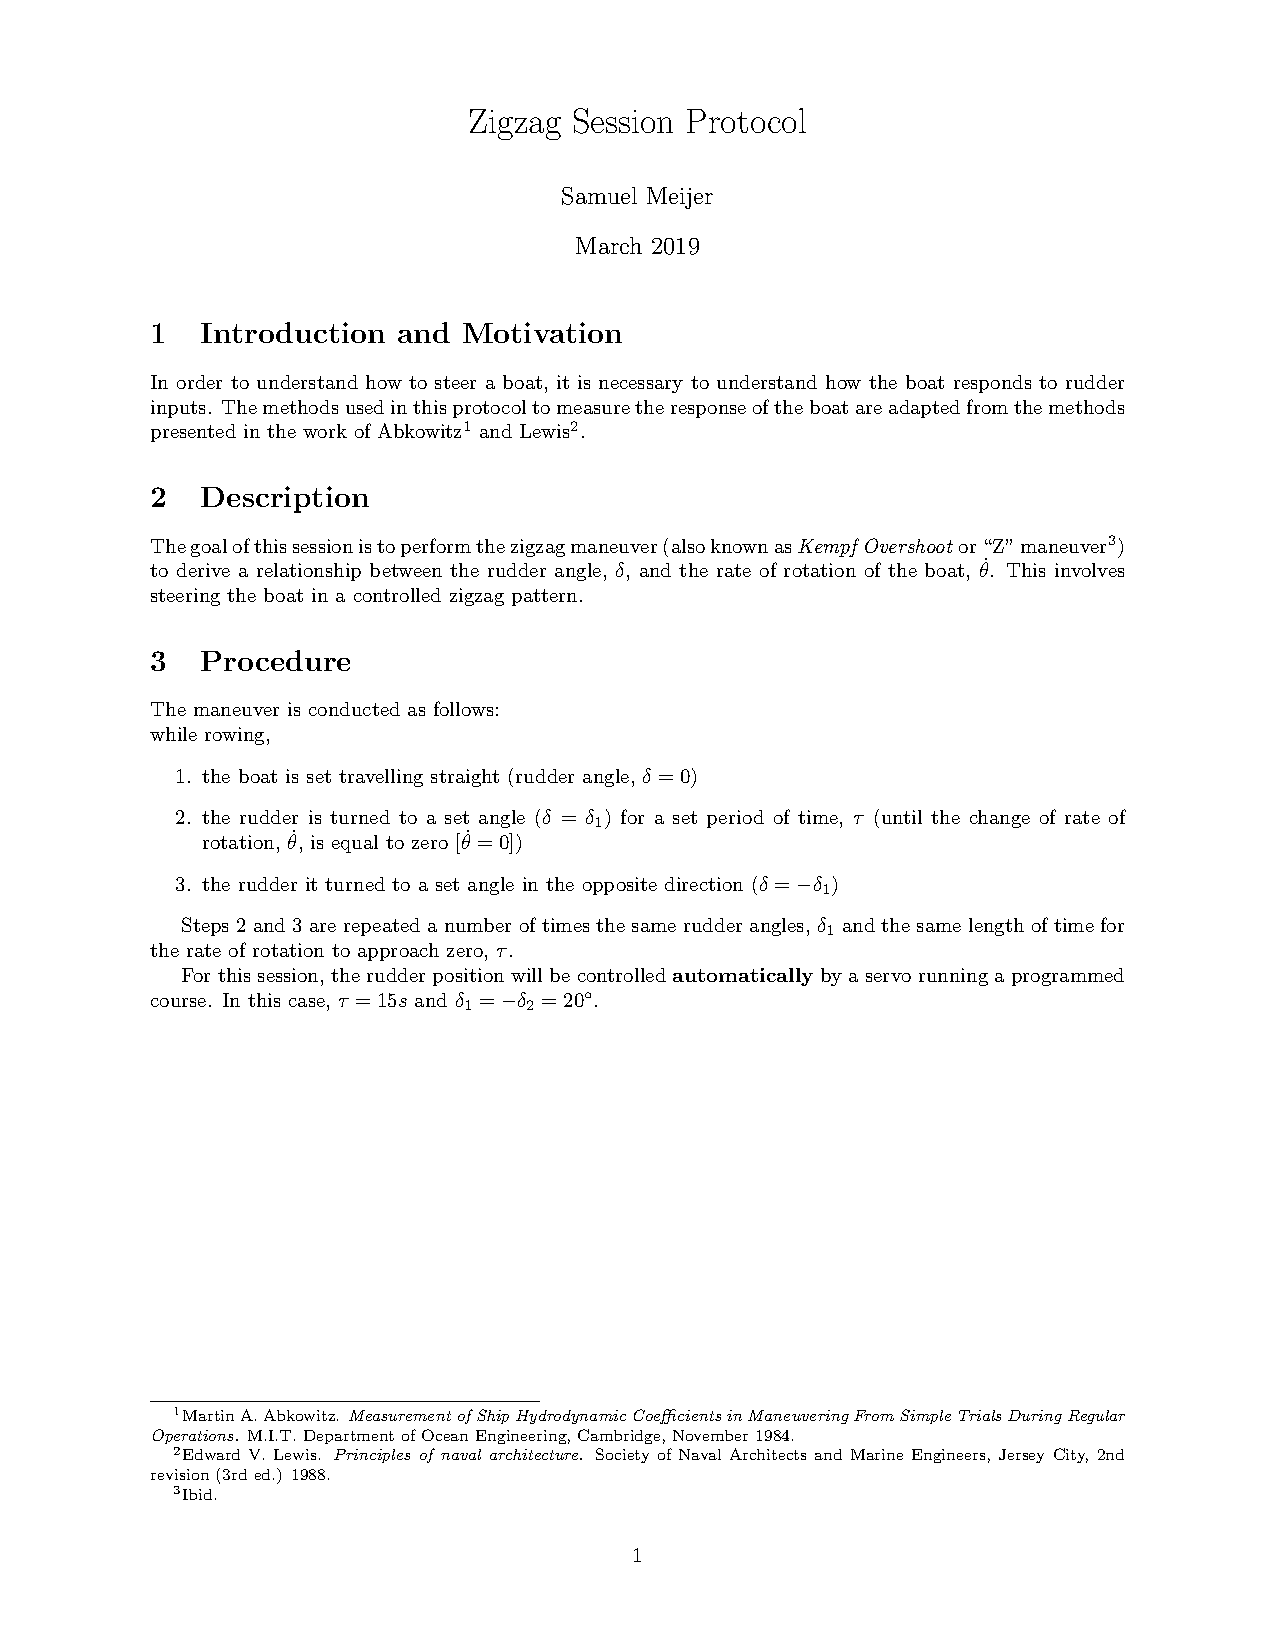
\includepdf[]{appendices/Session_Protocol-3.pdf}


\chapter{Predictive Modeling}

Feature Importance Analysis: Table showing feature importance scores from Random Forests/Gradient Boosting.

Hyperparameter Tuning: Explanation of hyperparameter optimization (e.g., GridSearchCV, RandomizedSearchCV).

Model Performance Metrics: Tables summarizing accuracy, precision, recall, F1-score, and ROC curves for different models.

Python Code Snippets: Machine learning model implementations.

\chapter{Additional Visualizations}

Cluster Interpretation: Heatmaps, scatter plots, and PCA biplots illustrating clustering results.
Regime Transitions: Graphs of detected volatility regimes over time.
Outlier Detection Results: Visualization of detected outliers using Mahalanobis distance.
Feature Correlation Matrix: Heatmap showing relationships between features.


\chapter{Computational Setup}

Software & Libraries Used: List of Python libraries (Pandas, NumPy, scikit-learn, TensorFlow, etc.).

Computing Environment: Python version, hardware specifications (if relevant for model training time).

Reproducibility Notes: Any considerations for ensuring code can be replicated.


\chapter{Supplementary Tables \& Results}

Descriptive Statistics: Summary statistics (mean, median, standard deviation, etc.) for key variables.

Extended Literature Review Tables: If applicable, tables summarizing related research findings.

Sensitivity Analysis: Results of robustness checks (e.g., how different parameter choices affect model outputs).



%%%%%%%%%%%%%%%%%%%%%%%%%%%%%%%%%%%%%%%%%%%
% Bibliography
%%%%%%%%%%%%%%%%%%%%%%%%%%%%%%%%%%%%%%%%%%%

\bibliographystyle{ieeetr}

\bibliography{references}


\end{document}